\documentclass[12pt]{report}

\usepackage[T1]{fontenc}
\usepackage[italian]{babel}
\usepackage[hidelinks]{hyperref}
\usepackage{tikz, pgfplots}
\usepackage{graphicx}
\usepackage{tabularx}

\hypersetup {
    colorlinks=true,
    urlcolor=blue,
    linkcolor=blue
}

% --------------- STYLE ---------------
\usepackage[margin=1.25in]{geometry}
\usepackage{xcolor}

\usepackage{fancyhdr}
\usepackage[Sonny]{fncychap}
\usepackage[most]{tcolorbox}

% Font
\renewcommand{\familydefault}{\sfdefault}
\usepackage{sansmath}
\sansmath

\pagestyle{fancy}
\setlength{\headheight}{15pt}
\rhead{\thepage}


% --------------- MATH ---------------
\usepackage{amsmath, amssymb, amsthm, amsfonts, mathtools}

\usepackage{mdframed}
\newtheoremstyle{th_style}
{0pt}{0pt}
{\normalfont}
{}
{\color{green!40!black}}
{\;}{0.25em}
{\thmname{\textbf{#1}}\thmnumber{ \textbf{#2}}{\color{black}\thmnote{\textbf{ -- #3}}}}

\newmdenv[
	rightline=false,
	leftline=true,
	topline=false,
	bottomline=false,
	linecolor=green!40!black,
	innerleftmargin=5pt,
	innerrightmargin=5pt,
	innertopmargin=5pt,
	innerbottommargin=5pt,
	leftmargin=0cm,
	rightmargin=0cm,
	linewidth=4pt
]{dBox}

\newmdenv[
	rightline=false,
	leftline=true,
	topline=false,
	bottomline=false,
	linecolor=green!40!black,
	backgroundcolor=black!5,
	innerleftmargin=5pt,
	innerrightmargin=5pt,
	innertopmargin=5pt,
	innerbottommargin=5pt,
	leftmargin=0cm,
	rightmargin=0cm,
	linewidth=4pt
]{pBox}

\theoremstyle{th_style}
\newtheorem{theoremeT}{Teorema}[chapter]
\newtheorem{definitionT}{Definizione}[chapter]
\newtheorem{propertyT}{Proprietà}[chapter]
\newtheorem{propositionT}{Proposizione}[chapter]
\newtheorem{corollaryT}{Corollario}[chapter]
\newtheorem{lemmaT}{Lemma}[chapter]
\newtheorem{observation}{Osservazione}[chapter]
\newtheorem{exampleT}{Esempio}[section]

\newenvironment{theorem}{\begin{pBox}\begin{theoremeT}}{\end{theoremeT}\end{pBox}}
\newenvironment{definition}{\begin{dBox}\begin{definitionT}}{\end{definitionT}\end{dBox}}
\newenvironment{property}{\begin{dBox}\begin{propertyT}}{\end{propertyT}\end{dBox}}
\newenvironment{proposition}{\begin{pBox}\begin{propositionT}}{\end{propositionT}\end{pBox}}
\newenvironment{corollary}{\begin{pBox}\begin{corollaryT}}{\end{corollaryT}\end{pBox}}
\newenvironment{lemma}{\begin{pBox}\begin{lemmaT}}{\end{lemmaT}\end{pBox}}
\newenvironment{example}{\begin{dBox}\begin{exampleT}}{\end{exampleT}\end{dBox}}


\pgfplotsset{compat=newest}

\newcommand{\N}{\mathbb{N}}
\newcommand{\Z}{\mathbb{Z}}
\newcommand{\R}{\mathbb{R}}
\newcommand{\RR}{\mathcal{R}}
\newcommand{\C}{\mathcal{C}}
\newcommand{\F}{\mathbb{F}}
\newcommand{\K}{\mathcal{K}}
\newcommand{\B}{\mathcal{B}}

\newcommand{\tx}{\tilde{x}}
\newcommand{\norm}[1]{\left\lVert#1\right\rVert}
\newcommand{\start}{\triangleright}

\DeclareMathOperator{\sign}{sign}
\DeclareMathOperator{\trn}{trn}
\DeclareMathOperator{\arr}{arr}
\DeclareMathOperator{\fl}{fl}
\DeclareMathOperator{\dist}{dist}
\DeclareMathOperator{\Ker}{Ker}
\DeclareMathOperator{\diag}{diag}
\DeclareMathOperator{\nnz}{nnz}
\DeclareMathOperator{\Var}{Var}

\title{Elementi di calcolabilità e complessità}
\author{Federico Bustaffa}
\date{15/04/2024}

\begin{document}

\maketitle

\begin{abstract}
	Lo scopo di questi appunti è rendere la comprensione dei
	concetti spiegati all'interno del corso il più semplice
	possibile fornendo esempi e spiegazioni quasi ad un livello
	divulgativo per quanto mi sia possibile.

	Non mancheranno il rigore e i formalismi spiegati a lezione
	una volta definite le basi per poterli comprendere.

	Ovviamente questi appunti rispecchiano la mia personale
	interpretazione dei concetti mostrati all'interno del corso
	e dunque anche i miei limiti di apprendimento degli stessi.

	Il corso sarà suddiviso in due parti: la prima tratterà la
	teoria della \textbf{calcolabilità}, mentre la seconda la
	teoria della \textbf{complessità}.
\end{abstract}

\tableofcontents

% -------------- CALCOLABILITA' -------------------
\part{Calcolabilità}

\chapter{Introduzione alla calcolabilità}
Iniziamo con la \textbf{teoria della calcolabilità} la quale
si pone come obbiettivo quello di definire cosa siano problemi,
funzioni e algoritmi, cercando di dare una definizione formale
di questi ultimi. Una volta definiti questi concetti sarà di
nostro interesse capire quali sono i problemi
\textbf{calcolabili} e quali invece no.

In questa prima parte non è di nostro interesse tenere di conto
le limitazioni che hanno i calcolatori reali. Ragioneremo quindi
supponendo che non questi non abbiamo limiti in tempo o spazio
per effettuare il calcolo.

Cercheremo quindi di capire quali sono i problemi
\textbf{calcolabili} mediante una \textbf{procedura effettiva},
quali invece \textbf{non} sono calcolabili per capire se ce ne
sono di interessanti, se ne esistono di reali o se sono solo
artificiali e puramente teorici.

\section{Algoritmo}

Cerchiamo ora di definire un algoritmo genetico sequenziale che sia una buona
base per quello che andremo a fare dopo. Si vuole infatti costruire un modello
su cui basare le possibili implementazioni che andremo a studiare.

\subsection{API e utilizzo}

Per quanto riguarda l'API messa a disposizione dell'utente vogliamo un qualcosa
che sia il più semplice possibile e che prevenga errori o cattiva gestione
delle strutture dati, fondamentali per la corretta esecuzione dell'algoritmo.

L'idea sarebbe quella di istanziare l'algoritmo come un oggetto, al quale
verranno forniti i vari metodi che compongono un algoritmo genetico.

\begin{minted}{py}
from genetic import GeneticAlgorithm

if __name__ == "__main__":
	ga = GeneticAlgorithm(
		population_size
		gen_func,
		selection_func,
		crossover_func,
		mutation_func,
		fitness_func,
		replacement_func,
		convergence_func
	)

	ga.run()
	results = ga.get()
\end{minted}

In questo modo non si espongono le strutture dati all'esterno della classe se
non come copie o come \emph{viste} dell'originale. Questo rende anche possibile
il riutilizzo di strutture dati già allocate andando rendere più efficiente
l'algoritmo in un senso che sarà più chiaro andando avanti.

\subsection{Cromosomi}

Prima di definire le varie fasi dell'algoritmo, introduciamo brevemente come
vengono rappresentati i \textbf{cromosomi}.

\begin{minted}{py}
class Chromosome:
	def __init__(self, values, fitness) -> None:
		self.values = values
		self.fitness = fitness
\end{minted}

Ogni cromosoma rappresenta un individuo della popolazione, il quale è
generalmente identificato da un vettore di valori numerici e da un valore di
fitness.

Noi tratteremo solo casi in cui abbiamo vettori numerici, sarà poi compito del
programmatore mappare il cromosoma in ciò che gli serve per risolvere il
problema di interesse.

\subsection{Generazione della popolazione iniziale}

In questa prima fase andiamo a generare una popolazione iniziale di $N$
individui in modo del tutto casuale. Evitare di generare duplicati è buona
norma, almeno in questa fase, così da garantire un alto grado di
\emph{biodiversità} iniziale.

\begin{minted}{py}
def __generate(self) -> None:
	for i in range(N):
		values = self.gen_func()
		while values in population:
			values = self.gen_func()
		self.population[i].values = values
\end{minted}

Per la fase iniziale di generazione, lasciamo al programmatore il compito di
definire come viene generato il singolo cromosoma. Sarà poi il modulo ad
occupersi di gestire i duplicati e memorizzare la popolazione.

\subsection{Selezione}

Le possibili implementazioni della fase di selezione degli individui per
l'accoppiamento sono molto varie e potrebbero non avere parti in comune.

Prendiamo ad esempio la selezione a \emph{torneo} in cui si scelgono a due a
due degli individui e quello con fitness più alta viene scelto.

In una soluzione a \emph{roulette} invece gli individui vengono scelti
singolarmente e volta per volta. In ogni caso si lavora sempre sull'intera
popolazione e non ci sono parti facilmente \emph{generalizzabili}.

Ecco perché in questa fase si richiede al programmatore di implementare la fase
di selezione per intero.

\begin{minted}{py}
def __selection(self):
	self.selected = self.selection_func(self.population)
\end{minted}

Ciò che si richiede è che la funzione di selezione ritorni una lista di
puntatori agli individui selezionati.

\subsection{Crossover}

La fase di crossover si rivelerà essere una delle più costose ed è quindi
necessario implementare delle ottimizzazioni già nella progettazione
dell'algoritmo sequenziale.

Per la fase di crossover facciamo alcune assunzioni, necessarie per riuscire
a parallelizzare l'algoritmo in seguito. Vogliamo infatti lasciare al
programmatore solamente il compito di definire l'operatore di crossover, il
quale prende in input solo due individui e restituisce (in genere due) nuovi
individui. Il come vengono formate le coppie viene lasciato alle routine
interne della classe che stiamo definendo.

\begin{minted}{py}
def __crossover(self) -> None:
	for i in range(0, len(self.selected), 2):
		father, mother = random.choices(self.selected, k=2)

		offspring1, offspring2 = self.crossover_func(father, mother)
		self.offsprings[i] = offspring1
		self.offsprings[i+1] = offspring2

		self.selected.remove(father)
		try:
			selected.remove(mother)
		except ValueError:
			pass
\end{minted}

Altra assunzione che fa l'algoritmo in questione è che il numero di nuovi
individui generati non cambia mai. Questo ci permette di inizializzare una
lista \verb|offsprings| a cui poi possiamo accedere tramite indice e senza
quindi andare riallocare di continuo memoria per i nuovi individui generati.

\subsection{Mutazione}

Per quanto riguarda la fase di mutazione si lascia al programmatore il compito
di definire una funzione che prende in input un cromosoma e applica una qualche
tecnica di mutazione.

\begin{minted}{py}
def __mutation(self) -> None:
	for i in range(len(self.offsprings)):
		if random.random() < self.mutation_rate:
			self.offsprings[i] = self.mutation_func(self.offsprings[i])
\end{minted}

Il modulo si occupa di gestire la probabilità che ogni individuo ha di essere
mutato.

\subsection{Valutazione}

Fase abbastanza semplice ma che costituisce uno dei colli di bottiglia maggiori
per le prestazioni

\begin{minted}{py}
def __evaluation(self) -> None:
	for i in range(len(self.offsprings)):
		self.offsprings[i].fitness = self.fitness_func(self.offsprings[i].values)
\end{minted}

Anche qui l'algoritmo non fa altro che applicare la funzione di fitness definita
dall'utente ad ogni nuovo individuo della popolazione.


\section{Macchine di Turing}

\section{Funzione di transizione}
La \textbf{funzione di transizione} $\delta$ è necessaria a
far progredire il calcolo. Come possiamo vedere dalla
definizione che ne abbiamo dato, questa prende in input una
coppia di valori.
\begin{itemize}
	\item Lo \textbf{stato corrente} $q$ della macchina.
	\item Un simbolo $\sigma$ dell'alfabeto
\end{itemize}

Notiamo inoltre che la funzione $\delta$ prende in input una
coppia di valori ma ritorna una tripla composta da uno stato
$q'$, che può essere anche $h$ in caso il calcolo sia terminato
con successo, un simbolo $\sigma'$ e una tra le 3 mosse $L$,
$R$ e $-$.

Ad ogni passo del calcolo, $\delta$ elabora la coppia in input
e restituisce una tripla contente il nuovo stato, il nuovo
simbolo da scrivere alla posizione attuale del cursore e come
ci si deve muovere al passo successivo.

Qualcuno potrebbe aver notato la similitudine con un automa a
stati finiti. In quanto vi è sempre uno stato corrente e, in
base a quello e ad una nuova parte dell'input ci si muove in
un nuovo stato o si rimane nello stesso. Non è tuttavia
corretto dire che una MdT è un automa.

\subsection{Considerazioni}
Ora che abbiamo le idee più chiare, facciamo qualche
considerazione in più su $\delta$. Essa è \textbf{iniettiva},
vale cioè che, prese due triple $(q', \sigma', D')$ e
$(q'', \sigma'', D'')$ tali che
\begin{gather*}
	\delta (q, \sigma) =  (q', \sigma', D') \\
	\delta (q, \sigma) = (q'', \sigma'', D'')
\end{gather*}
allora $q' = q''$, $\sigma' = \sigma''$ e $D' = D''$.
Questo ci dice sostanzialmente che, dato uno stato e un simbolo
c'è un solo altro stato in cui possiamo andare. Un'altra cosa
da specificare è che per $\delta$ vale sempre che se
\[ \delta(q, \start) = (q', \sigma, D) \]
allora $\sigma = \start$ e $D = R$. Questo ci dice che se ci
troviamo all'inizio del nastro possiamo andare solo a destra.

Ritornando velocemente
all'\hyperref[sec: algoritmo]{idea intuitiva di algoritmo},
possiamo facilmente verificare la prima e seconda condizione
sono verificate poiché, sia $Q$ che $\Sigma$ sono insiemi
finiti e di conseguenza anche $\delta$ contiene un numero
finito di elementi.

\subsection{Alfabeto}
I dati su cui opera una MdT sono stringhe $w$ di caratteri
appartenenti a $\Sigma$, più precisamente $w \in \Sigma^*$,
dove $\Sigma^*$ comprende anche la stringa vuota $\epsilon$.

Senza stare a incasinarsi con inutili formalismi matematici,
se $\Sigma$ è l'alfabeto, allora $\Sigma^*$ è l'insieme di
tutte le possibili stringhe generabili con quell'alfabeto e
la stringa vuota.

\begin{example}
	Prendiamo ad esempio l'alfabeto binario
	\begin{gather*}
		\Sigma = \{ 0, 1 \} \\
		\Downarrow \\
		\Sigma^* = \{ \epsilon, 0, 1, 01, 10, 11, \dots \}
	\end{gather*}
\end{example}
\section{Computazione}
Finalmente vediamo come opera una MdT su qualche problema di
esempio. La \textbf{configurazione corrente} di una MdT viene
identificata $(q, u, \sigma, v)$ dove
\begin{itemize}
	\item $q$ è lo stato corrente.
	\item $u$ è la stringa a sinistra del carattere attuale.
	\item $\sigma$ è il carattere attuale.
	\item $v$ è il resto della stringa che termina con un
	      carattere non nullo.
\end{itemize}
La situazione corrente di una MdT può essere espressa più
comodamente con $(q, u \underline{\sigma} v)$. Graficamente
una MdT appare in questo modo
\begin{center}
	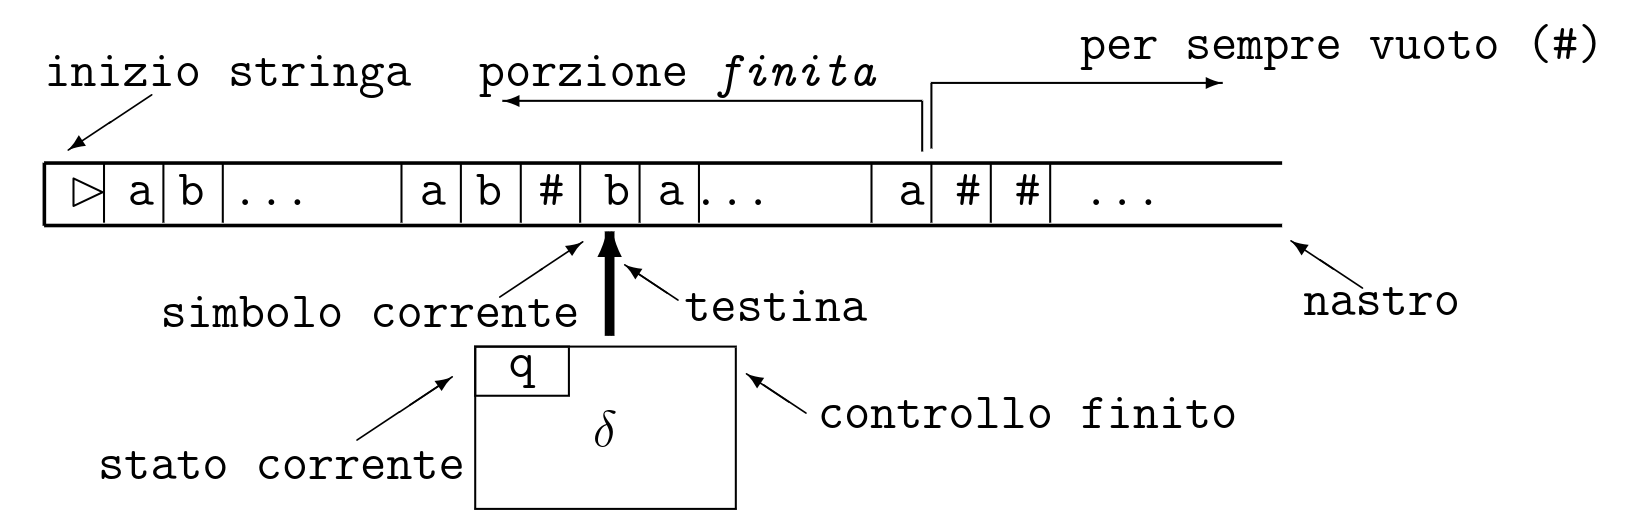
\includegraphics[scale=0.225]{images/turing.png}
\end{center}
Tenendo a mente questa figura possiamo provare a costruire la
nostra prima MdT.

\begin{example} \label{ex: 11}
	Vogliamo costruire una MdT in grado di dirci se la stringa
	binaria in input contiene una sottosequenza composta da
	due $1$ consecutivi.

	Per costruire la nostra macchina abbiamo bisogno di due
	stati ($q_0$ e $q_1$), di due simboli ($0$ e $1$) e di
	una funzione di transizione $\delta$.

	Per capire se la stringa in input contiene almeno una
	sottostringa composta da due $1$ consecutivi, iniziamo
	con lo stato iniziale $q_0$, il quale indica sia lo stato
	inziale della macchina sia lo stato in cui la macchina
	deve transire ogni qual volta incontra uno $0$.

	Abbiamo poi bisogno di uno stato $q_1$ in cui la macchina
	transisce quando incontra un $1$ nella sequenza dopo essere
	stata in uno stato $q_0$.

	Se ci troviamo nello stato $q_1$ e incontriamo un altro $1$
	la macchina transisce nello stato $h$ di terminazione. La
	funzione $\delta$ di transizione che deriva dai seguenti
	ragionamenti è la seguente
	\begin{center}
		\begin{tabular}{|c|c|c|}
			\hline
			$q$   & $\sigma$ & $\delta(q, \sigma)$ \\
			\hline
			$q_0$ & $\start$ & $q_0, \start, R$    \\
			$q_0$ & $0$      & $q_0, \#, R$        \\
			$q_0$ & $1$      & $q_1, \#, R$        \\
			$q_1$ & $0$      & $q_0, \#, R$        \\
			$q_1$ & $1$      & $h, \#, -$          \\
			\hline
		\end{tabular}
	\end{center}
	Come possiamo notare, ogni volta che incontriamo un
	carattere lo "cancelliamo" scrivendo $\#$ ma avremmo potuto
	lasciare il numero che incontravamo. Vediamo una possibile
	simulazione di esecuzione con la seguente stringa binaria
	in input
	\[ 01011 \]
	La nostra configurazione iniziale è
	\[ q_0 / \underline{\start} 01011 \]
	dove il simbolo sottolineato è quello su cui si trova il
	cursore. La sequenza di operazioni sarà quindi la seguente
	\begin{align*}
		q_0 / & \underline{\start} 01011       \\
		q_0 / & \start \underline{0} 1011      \\
		q_0 / & \start \# \underline{1} 011    \\
		q_1 / & \start \#\# \underline{0} 11   \\
		q_0 / & \start \#\#\# \underline{1} 1  \\
		q_1 / & \start \#\#\#\# \underline{1}  \\
		h /   & \start \#\#\#\# \underline{\#}
	\end{align*}
	Il calcolo è dunque terminato con successo.
\end{example}

Per vedere una MdT in azione è possibile visitare questo
\href{https://turingmachinesimulator.com/}{sito} in cui è
possibile programmare una MdT oppure eseguire esempi già
proposti.

\subsection{Configurazione e computazione}
Come abbiamo detto precedentemente, una \textbf{configurazione}
è definita dalla quadrupla
\[ \gamma = (q, u, \sigma, v) \]
Ciò che non abbiamo detto è che gli elementi di $\gamma$
appartengono al seguente insieme
\[
	\gamma \in (Q \cup \{ h \}) \times
	\Sigma^* \times \Sigma \times \Sigma^F
\]
L'ultimo insieme ($\Sigma^F$) è un po' particolare, è infatti
definito come
\[
	\Sigma^F = \Sigma^* \cdot \left( \Sigma \backslash
	\{ \# \} \right) \cup \{ \epsilon \}
\]
quindi possiamo scrivere la stringa $v$ come
$\sigma_0 \sigma_1 \dots \sigma_n$, con $\sigma_n \neq \#$,
al posto della stringa infinita composta dai vari $\sigma$ e
con infiniti $\#$ alla fine.

Si noti però che un qualsiasi carattere $\sigma_i$ con $i < n$
può essere $\#$ ed inoltre la stringa $u$ può essere vuota
solo quando il carattere corrente è $\start$. La convenzione
impone quindi di scrivere la configurazione iniziale del primo
esempio fatto, in questo modo
\[ (q_0, \start 01011, \epsilon) \]

\begin{definition}
	Una \textbf{computazione} è una successione finita di
	passi
	\[ (q_0, w) \to^* (q', w') \]
	dove $\to^*$ è la chiusura riflessiva e transitiva di
	$\to$. Ovviamente se vi sono $n$ passi, la computazione
	è lunga $n$ e dunque scriveremo $\to^n$.
\end{definition}

Definiamo meglio cos'è un \textbf{passo di computazione},
procedendo per casi e considerando $a$, $b$ e $c$ come elementi
generici di $\Sigma$.
\begin{itemize}
	\item $(q, u \underline{a} v) \to (q', u \underline{b} v)$
	      se $\delta (q, a) = (q', b, -)$.
	\item $(q, u c \underline{a} v) \to
		      (q', u \underline{c} b v)$
	      se $\delta (q, a) = (q', b, L)$.
	\item \begin{enumerate}
		      \item $(q, u \underline{a} c v) \to
			            (q', u b \underline{c} v)$
		            se $\delta (q, a) = (q', b, R)$.
		      \item $(q, u \underline{a}) \to
			            (q', u b \underline{\#})$
		            se $\delta (q, a) = (q', b, R)$.
	      \end{enumerate}
\end{itemize}
In questo modo garantiamo che ciascun passo abbia effetto
limitato sulle configurazioni, come richiesto dalla seconda
parte del punto 2 nell'\hyperref[sec: algoritmo]{idea intuitiva
	dell'algoritmo}.

Allo stesso modo possiamo immaginarci che se partiamo da uno
stato iniziale $(q_0, \underline{\start} w)$, dopo un certo
numero di passi arriviamo in uno stato $(q', w')$.

\begin{definition} \label{def: convergenza}
	Diciamo che una computazione \textbf{termina} o
	\textbf{converge} ($\downarrow$) se e solo se lo stato
	finale è $h$. Nell'esempio \ref{ex: 11} fatto qui sopra
	$q' = h$.

	Diciamo invece che la computazione \textbf{non termina}
	o \textbf{diverge} ($\uparrow$) se e solo se per ogni
	$q'$ e $w'$ tali che
	\[ (q_0, w) \to^* (q', w') \]
	esistono $q''$ e $w''$ tali che
	\[ (q', w') \to^* (q'', w'') \]
	ovvero tali che è sempre possibile fare un nuovo passo di
	computazione.
\end{definition}

Come possiamo vedere, le MdT definite in questo modo,
rispettano l'idea intuitiva di algoritmo che abbiamo dato
all'inizio.

\begin{example} \label{ex: non termina}
	Facciamo un esempio di computazione che non termina mai
	tramite una macchine che semplicemente non contiene il
	simbolo $h$ di terminazione.
	\begin{center}
		\begin{tabular}{|c|c|c|}
			\hline
			$q$   & $\sigma$ & $\delta$             \\
			\hline
			$q_0$ & $\start$ & $q_0$, $\start$, $R$ \\
			$q_0$ & $a$      & $q_0$, $a$, $R$      \\
			$q_0$ & $\#$     & $q_0$, $\#$, $R$     \\
			\hline
		\end{tabular}
	\end{center}
\end{example}

Proviamo ora a fare un esempio più concreto di una MdT che
calcola qualcosa di più sensato rispetto agli esempi visti
fino ad ora.

\begin{example}
	Questa MdT si propone di calcolare la somma di due numeri
	$n$ ed $m$, dove $n$ ed $m$ sono rappresentati in notazione
	unaria tramite il simbolo $|$ ripetuto $n$ (o $m$) volte.
	La funzione $\delta$ è definita dalla seguente tabella
	\begin{center}
		\begin{tabular}{|c|c|c|}
			\hline
			$q$   & $\sigma$ & $\delta$         \\
			\hline
			$q_0$ & $\start$ & $q_0, \start, R$ \\
			$q_0$ & $|$      & $q_0, |, R$      \\
			$q_0$ & $+$      & $q_1, |, R$      \\
			$q_1$ & $|$      & $q_1, |, R$      \\
			$q_1$ & $\#$     & $q_2, \#, L$     \\
			$q_2$ & $|$      & $h, \#, -$       \\
			\hline
		\end{tabular}
	\end{center}
	Il simbolo $+$ deve essere tra le due sequenze di $|$.
	Proviamo ora ad eseguire la computazione per il calcolo
	di $1 + 2$, partendo dalla configurazione iniziale
	\[ q_0/ \quad \underline{|} + | | \]
	Svolgiamo quindi i seguenti passi
	\begin{gather*}
		(q_0, \; \underline{\start} | + | | ) \to
		(q_0, \; \start \underline{|} + | | ) \\
		(q_0, \; \start \underline{|} + | | ) \to
		(q_0, \; \start | \underline{+} | | ) \\
		(q_0, \; \start | \underline{+} | | ) \to
		(q_1, \; \start | | \underline{|} | ) \\
		(q_1, \; \start | | \underline{|} | ) \to
		(q_1, \; \start | | | \underline{|} ) \\
		(q_1, \; \start | | | \underline{|} ) \to
		(q_1, \; \start | | | | \underline{\#} ) \\
		(q_1, \; \start | | | | \underline{\#} ) \to
		(q_2, \; \start | | | \underline{|} \# ) \\
		(q_2, \; \start | | | \underline{|} \# ) \to
		(h, \; \start | | | \underline{\#} \# )
	\end{gather*}
	per concludere che il calcolo termina dato che siamo
	giunti nello stato speciale $h$. Come possiamo vedere il
	nostro risultato è dato dal numero di $|$ rimanente.
\end{example}

Un altro tipico esempio di utilizzo di queste macchine è
quello di decidere se una stringa è palindroma. In questo
caso descriviamo brevemente quale sarebbe l'idea.
\begin{enumerate}
	\item Si controlla il primo carattere della stringa, lo si
	      sovrascrive con $\start$ e si passa in uno stato
	      specifico per quel carattere (supponendo che il primo
	      carattere sia $a$, si passa in $q_a$).
	\item Si arriva in fondo alla stringa e si controlla che
	      l'ultimo carattere sia uguale al primo, se sì, lo
	      si sovrascrive con un $\#$.
	\item Si torna indietro fino al primo $\start$ che si
	      incontra.
\end{enumerate}
Si ripete il procedimento finché non si esaurisce tutta la
stringa o finché non fallisce.

\section{Sintassi}
Il \textbf{lambda calcolo} può essere visto come il primo \textbf{linguaggio funzionale} e consente di definire
solo funzioni anonime con una sintassi minimale e molto semplice.

Un programma nel lambda calcolo è di fatto un'espressione, detta \textbf{lambda espressione}, la cui sintassi ha
3 componenti principali:
\begin{itemize}
	\item \textbf{Identificatori}
	      \[ e ::= x \]
	      In questo modo l'\textbf{identificatore} $x$ assume come valore l'espressione $e$.
	\item \textbf{Astrazione funzionale}
	      \[ \lambda x.e \]
	      Indica una funzione (anonima) con parametro $x$ e corpo $e$.
	\item \textbf{Applicazione funzionale}
	      \[ e_1 \; e_2 \]
	      In questo modo si applica l'espressione $e_1$ al parametro $e_2$.
\end{itemize}
Una funzione può essere definita e applicata scrivendo tutto nella solita riga.
\[ (\lambda x.(\lambda y.xy)) \quad (\lambda z.z) \]

\subsection{Costruttore lambda}
Lo \textbf{scope} del lambda si estende il più a destra possibile. Scrivere
\[ \lambda x. \lambda y. x y \]
equivale a
\[ \lambda x. (\lambda y. (x y)) \]
In entrambi i casi stiamo definendo una funzione che prende $x$ come parametro e come corpo ha una funzione con
parametro $y$ e corpo l'applicazione di $x$ a $y$, ovvero $xy$.

\subsection{Applicazione funzionale}
L'\textbf{applicazione funzionale} associa a sinistra. Scrivere
\[ e_1 e_2 e_3 \]
è come scrivere
\[ (e_1 e_2) e_3 \]
In entrambi i casi stiamo applicando $e_3$ all'applicazione di $e_1$ su $e_2$.

\subsection{Variabili legate e libere}
Tutte le altre variabili che non sono associate a una dichiarazione con un qualche $\lambda$ sono \textbf{libere}.

Le variabili in una lambda espressione che sono introdotte (dichiarate) in un qualche $\lambda$ sono
\textbf{legate} da quel $\lambda$.

\subsubsection{Insieme delle variabili libere}
L'\textbf{insieme delle variabili libere} di una lambda espressione $e$, denotato come $FV(e)$, è definito
ricorsivamente sulla struttura di $e$ come segue:
\begin{gather*}
	FV(x) = \{ x \} \\
	FV(\lambda x.e) = FV(e) \backslash \{ x \} \\
	FV(e_1 e_2) = FV(e_1) \cup FV(e_2)
\end{gather*}
In altre parole il calcolo di $FV(e)$ scende ricorsivamente accumulando tramite l'unione tutte le variabili che
incontra nelle sottoespressioni. Nel momento in cui si incontra una $\lambda$-astrazione la variabile legata
viene rimossa dall'insieme delle variabili libere.
\section{Semantica}
Prima di addentrarci nelle dinamiche del linguaggio appena
definito, dobbiamo definire la \textbf{memoria}. Nel nostro
caso lo facciamo tramite la funzione
\[ \sigma : \Var \to \N \]
che, data una variabile in input, restituisce il suo valore
in memoria (operazione di lettura). Noi però siamo interessati
anche a modificare la memoria, definiamo quindi l'operazione
di \textbf{aggiornamento} tramite la funzione, o meglio il
funzionale a tre argomenti
\[
	- [ - / - ] : (\Var \to \N) \times
	\N \times \Var \to (\Var \to \N)
\]
che è definita come
\[
	\sigma [n / x](y) = \begin{cases}
		n         & \text{se } y = x  \\
		\sigma(y) & \text{altrimenti}
	\end{cases}
\]
e cambia il valore della variabile $x$ con $n$. Quando
cercheremo di accedere nuovamente alla variabile $x$ in
memoria, la funzione $\sigma$ ci ritornerà il valore aggiornato.

La \textbf{semantica} di un'espressione aritmetica è data
dalla seguente funzione di \textbf{valutazione}, in cui andremo
a scrivere il suo argomento principale, l'espressione aritmetica,
tra le parentesi $[[$ e $]]$, cui viene giustapposto il secondo
argomento, cioè la memoria in cui l'espressione va valutata.
\[ \xi [[-]] - : E \times (\Var \to \N) \to \N \]
Proviamo a capire come questa funzione si comporta quando
prende in input espressioni aritmetiche.
\begin{align*}
	\xi [[n]] \sigma              & = n         \\
	\xi [[x]] \sigma              & = \sigma(x) \\
	\xi [[E_1 + E_2]] \sigma      &
	= \xi [[E_1]] \text{ più } [[E_2]] \sigma   \\
	\xi [[E_1 \times E_2]] \sigma &
	= \xi [[ E_1 ]] \text{ per } [[E_2]] \sigma \\
	\xi [[E_1 - E_2]] \sigma      &
	= \xi [[ E_1 ]] \text{ meno } [[E_2]] \sigma
\end{align*}
Per adesso limitiamoci a notare che se diamo alla funzione di
valutazione un numero $n$, qualunque sia la memoria, questa
ci restituirà il numero stesso.

Se invece gli passiamo una variabile, questa ci restituirà
il valore della variabile in memoria, si fa infatti uso della
funzione $\sigma$.

Se invece passiamo una qualche operazione aritmetica, questa
verrà valutata come la somma (oppure sottrazione o prodotto)
delle valutazioni degli operandi.

\begin{example}
	Proviamo a valutare l'espressione
	\[ x \times 2 - ((y - 7) + 1) \]
	nella memoria $\sigma$ tale che
	\[ \sigma (x) = 3 \quad \text{e} \quad \sigma(y) = 5 \]
	I passaggi per risolvere l'esercizio sono i seguenti
	\begin{align*}
		  & \xi [[ x \times 2 - ((y - 7) + 1) ]] \sigma \\
		= & \xi [[ x \times 2 ]] \sigma \text{ meno }
		\xi [[ (y - 7) + 1 ]] \sigma
	\end{align*}
	come possiamo notare, quando c'è un'ambiguità tra le
	precedenze supponiamo di sapere quale sia l'ordine
	corretto. In questo caso valutiamo "prima" il meno.
	\begin{align*}
		= & (\xi [[ x ]] \sigma \text{ per } 2) \text{ meno }
		\xi [[ (y - 7) + 1 ]] \sigma                          \\
		= & (\sigma(x) \text{ per } 2) \text{ meno }
		\xi [[ (y - 7) + 1 ]] \sigma                          \\
		= & (3 \text{ per } 2) \text{ meno }
		\xi [[ (y - 7) + 1 ]] \sigma
	\end{align*}
	ora abbiamo semplicemente preso il valore $3$ dalla memoria
	per sostituirlo a $x$.

	\begin{align*}
		= & 6 \text{ meno } (\xi [[y - 7]] \sigma
		\text{ più } 1)                                  \\
		= & 6 \text{ meno } ((\xi [[y]] \text{ meno } 7)
		\text{ più } 1)                                  \\
		= & 6 \text{ meno } ((\sigma(y) \text{ meno } 7)
		\text{ più } 1)
	\end{align*}
	Di seguito $5 - 7 = 0$ perché stiamo utilizzando il
	\emph{meno ridotto}, il quale ritorna $0$ quando il
	minuendo è maggiore o uguale del sottraendo.
	\begin{align*}
		= & 6 \text{ meno } ((5 \text{ meno } 7)
		\text{ più } 1)                          \\
		= & 6 \text{ meno } (0 \text{ più } 1)   \\
		= & 6 \text{ meno } 1 = 5
	\end{align*}
	Il calcolo per il resto è abbastanza banale.
\end{example}

Passiamo ora alla semantica delle operazioni booleane, che
non si inventano nulla di diverso rispetto alle espressioni
aritmetiche. Semplicemente la funzione di valutazione è
definita in modo da restituire valori booleani.
\[ \B[[-]] - : \B \times (\Var \to \N) \to \text{Bool} \]
Come prima andiamo a vedere cosa succede per vari input a
tale funzione di valutazione.
\begin{align*}
	\B [[t]] \sigma            & = tt                           \\
	\B [[f]] \sigma            & = ff                           \\
	\B [[E_1 < E_2]] \sigma    & =
	\xi [[E_1]] \sigma \text{ minore } \xi [[E_2]] \sigma       \\
	\B [[\lnot B]] \sigma      & = \text{ not } \B [[B]] \sigma \\
	\B [[B_1 \lor B_2]] \sigma & = \B [[B_1]] \sigma
	\text{ or } \B [[B_2]] \sigma
\end{align*}
Lo stile di definizione seguito fino ad ora prende il nome di
stile \textbf{denotazionale} e si propone di associare una
funzione a ciascun operatore.

Ci sono vari modi per definire una semantica, noi per il
momento andremo a definire la semantica tramite un approccio
\textbf{operazionale}, ossia guidato dalla sintassi.

Quello che andremo a fare è definire una sorta di macchina
astratta che procede per passi discreti, apportando modifiche
discrete alle sue configurazioni o stati, che possiamo
immaginare come coppie $(\text{comando}, \sigma)$.

Tale macchina, che definisce la semantica di un linguaggio
di programmazione, prende il nome di
\text{sistema di transizioni} ed è identificato dalla coppia.
\[ (\Gamma, \to) \]
dove $\Gamma$ è la classe delle \emph{configurazioni} (nel
nostro caso sono coppie $(C, \sigma)$) e
$\to \subseteq \Gamma \times \Gamma$ è una funzione detta
\textbf{di transizione}.

Tale coppia definisce come il nostro programma evolve in base
ai comandi che dobbiamo eseguire e a come questi modificano
la memoria.

In realtà noi seguiremo un approccio di tipo
\textbf{Structural Operational Semantics} (o
\emph{small steps}), in cui ciascuna transizione
\[ (c, \sigma) \to (c', \sigma') \]
rappresenta un singolo passo di computazione, ossia la macchina
ha attraversato lo stato $(c, \sigma)$ e \emph{transisce} nello
stato $(c', \sigma')$.

Possiamo allora fare considerazioni del tutto analoghe a quelle
fatte per la MdT, ossia possiamo dire che una computazione è
la chiusura riflessiva e transitiva della funzione di
transizione. Formalmente
\[ (c, \sigma) \to^* (c', \sigma') \]
In questo caso una computazione termina (o converge) se
\[ (c, \sigma) \to^* \sigma' \]
Quello che si vuole è che la relazione descritta precedentemente
come \emph{passo di computazione} soddisifi i seguenti assiomi
e regole di inferenza
\begin{center}
	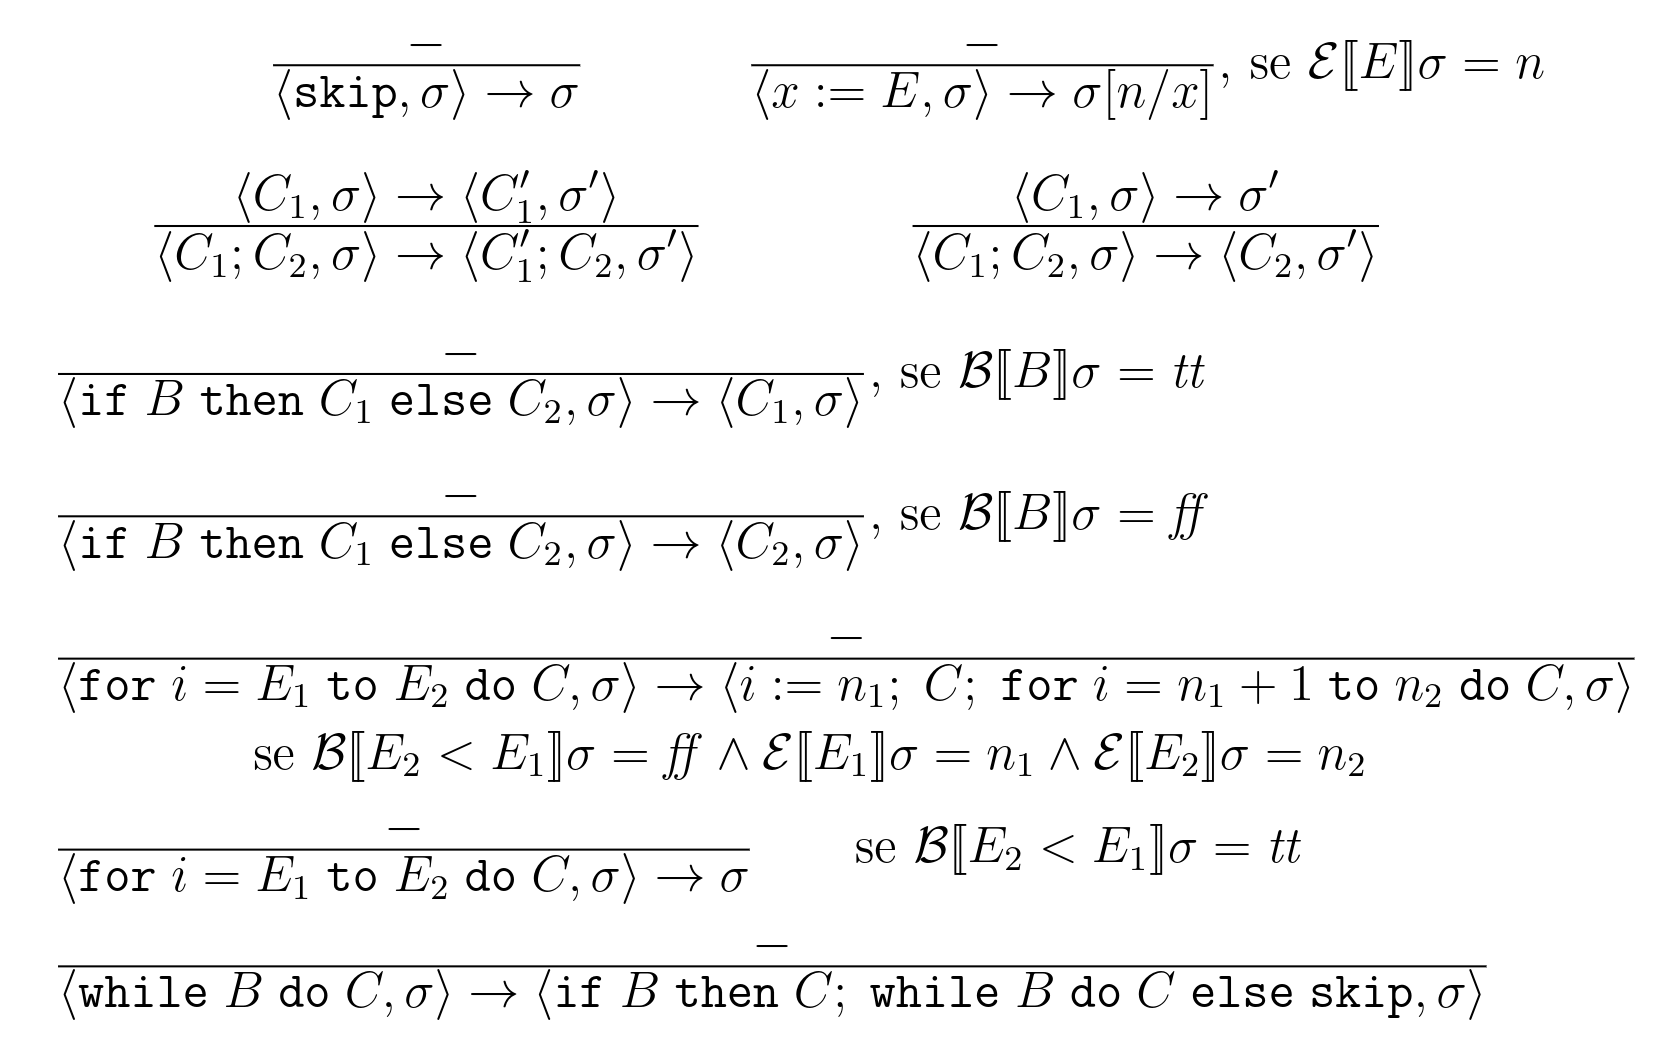
\includegraphics[scale=0.225]{images/assiomi.png}
\end{center}
Di particolare interesse è la regola di inferenza per
l'assegnamento, poiché chiarisce l'operazione di
\emph{aggiornamento} della memoria che avevamo lasciato in
sospeso.

Noi ci comportiamo come se la memoria fosse già inizializzata
per il nostro programma. Non ci sono vere e proprie operazioni
di scrittura della memoria. Ogni variabile esiste già in
essa e l'unica che cosa che ci è concesso fare è modificare il
suo valore.

Con la notazione $\sigma[n/x]$ intendiamo modificare il valore
della variabile $x$ presente in memoria con $n$. Stiamo in
realtà modificando la funzione che associa a $x$ un certo
valore (supponiamo $m$) con un altro valore ($n$).

La notazione che avevamo visto in precedenza per l'operazione
di aggiornamento significa che, se diamo $y$ in input a
$\sigma$ modificata, ossia $\sigma [n / x]$, se $y = x$,
allora stiamo in realtà cercando il valore di $x$ e dunque la
funzione ritorna $n$. Altrimenti stiamo cercando il valore di
$y$ presente in memoria e mai modificato dall'inizio
dell'esecuzione.

Per le altre regole teniamo a mente che, tutte quelle che
presentano una condizione a destra, si potrebbero scrivere
con la stessa condizione sopra.

In ogni caso per leggere le regole di inferenza seguiamo un
patter di questo tipo: se ci troviamo nello stato definito
descritto sotto la riga e a sinistra della freccia, si
transisce nello stato a destra della freccia se la condizione
è verificata.

\begin{example}
	Proviamo a dimostrare che il comando $C_1 ; C_2$ termina,
	tramite induzione.
	\begin{proof}
		Partiamo dalla regola di inferenza
		\[
			\frac{(C_1, \sigma) \to \sigma'}
			{(C_1 ; C_2, \sigma) \to (C_2 , \sigma')}
		\]
		e come ipotesi induttiva usiamo il fatto che se
		$C_1$ termina e $C_2$ termina, allora $C_1 ; C_2$
		termina. Se consideriamo la regola di inferenza
		\[
			\frac{(C_1, \sigma) \to (C_1', \sigma')}
			{(C_1 ; C_2, \sigma) \to (C_1' ; C_2 , \sigma')}
		\]
		il discorso è analogo con un passaggio in più. Se
		$C_1'$ termina ci ritroviamo al caso precedente e
		quindi anche $C_1 ; C_2$ termina.
	\end{proof}
\end{example}

\begin{example}
	Proviamo invece a dimostrare che il seguente programma
	\[ \text{while } tt \text{ do} \text{ skip}, \sigma \]
	non termina.
	\begin{proof}
		Per dimostrare che il programma non termina iniziamo
		a prendere la nostra configurazione di comandi e
		notiamo che corrisponde alla regola
		\[
			\frac{-}{(\text{while } B \text{ do } C, \sigma)
				\to (\text{if } B \text{ then } C;
				\text{ while } B \text{ do } C
				\text{ else skip}, \sigma )}
		\]
		che ci fa transire nello stato
		\[
			\text{if } tt \text{ then skip}, \sigma;
			\text{ while } tt \text{ do skip}, \sigma
			\text{ else skip}, \sigma
		\]
		a questo punto usiamo l'assioma dell'\verb|if| e
		otteniamo
		\[
			\text{skip}, \sigma ; \text{ while } tt
			\text{ do skip}, \sigma
		\]
		il primo comando è uno \verb|skip| e dunque ritorniamo
		al punto di partenza, ossia
		\[ \text{while } tt \text{ do} \text{ skip}, \sigma \]
		Ne concludiamo quindi che siamo entrati in un ciclo
		infinito.
	\end{proof}
\end{example}


\section{Problemi e funzioni}
Per il momento abbiamo usato i nostri costrutti per calcolare
una funzione (la somma per esempio) o per decidere
l'appartenenza di un elemento ad un insieme (decidere se una
stringa è palindroma).

In questa prima parte del corso andremo a definire meglio il
concetto di \textbf{problema} e di \textbf{funzione} che, nel
nostro caso, non hanno l'accezione cui siamo abituati.

Un esempio di \emph{problema} è la domanda: "qual è il massimo
comun divisore tra $x$ e $y$?". Se sostituiamo a $x$ e a $y$
dei valori, per esempio 34 e 98, otteniamo un \textbf{caso}
del problema.

\begin{definition}
	Siano $\Sigma$, $\Sigma_0$ e $\Sigma_1$ tali che
	\[ \#, \start \notin \Sigma_0 \cup \Sigma_1 \]
	e
	\[ ]\Sigma_0 \cup \Sigma_1 \subset \Sigma \]
	allora diciamo che una funzione
	\[ f : \Sigma_0 \to \Sigma_1 \]
	è \textbf{Turing calcolabile} o \textbf{T-calcolabile},
	se e solo se
	\begin{gather*}
		\forall w \in \Sigma_0^* : f(w) = z \\
		\Updownarrow \\
		(q_0, \underline{\start} w) \to_M^*
		(h, \start z \underline{\#})
	\end{gather*}
	Si dice anche che $f$ è T-calcolabile se esiste una MdT
	$M$ che la calcola.
\end{definition}

Ora che abbiamo la definizione precisa di cosa sia una
funzione T-calcolabile proviamo a fare una cosa analoga per
il linguaggio WHILE che abbiamo definito in precedenza.

\begin{definition}
	Diciamo che una funzione
	\[ f : \Var \to \N \]
	è \textbf{WHILE-calcolabile} oppure diciamo che un comando
	$C$ \textbf{calcola} $f$, se e solo se
	\begin{gather*}
		\forall \sigma \in \Var \to \N : f(x) = n \\
		\Updownarrow \\
		(C, \sigma) \to^* \sigma' \quad \land \quad
		\sigma'(x) = n
	\end{gather*}
\end{definition}

Notiamo che la variabile $x$ di input è anche la variabile
di output, ossia quella che contiene il risultato.

\subsection{Codifiche}
Ci chiediamo ora se per una funzione $f$ che non opera su
dati sotto formato di stringa, memorie o numeri naturali,
le nozioni di calcolabilità che abbiamo definito fino ad ora
sono ancora valide.

Se così non fosse dovremmo ridefinire ogni volta tali nozioni
per ogni dominio di ogni funzione con un formato differente da
quelli che abbiamo già incontrato.

Per superare il problema si fa uso di opportune
\textbf{codifiche} dei dati, ossia funzioni che svolgono
il seguente compito.
\begin{enumerate}
	\item Dato $x$ in formato $A$, lo si codifica in un formato
	      $B$ con cui riusciamo a calcolare.
	\item Si applica la MdT a $y$ e si ottiene il risultato $z$
	      (se la computazione termina) in formato $B$.
	\item Si traduce $z$ dal formato $B$ al formato $A$.
\end{enumerate}
D'ora in avanti considereremo solo i numeri naturali come i
nostri dati. Abbiamo però bisogno che la funzione di codifica
sia \emph{biunivoca}.

\begin{example}
	La seguente funzione codifica coppie di naturali come un
	singolo naturale ed è detta codifica a
	\textbf{coda di colomba}.
	\[ (x, y) \to \frac{1}{2} (x^2 + 2 x y + y^2 + 3 x + y) \]
	la cui decodifica, ossia la funzione inversa è la seguente
	\[
		n \to (n - \frac{1}{2} k \cdot (k + 1),
		k - (n - \frac{1}{2} k \cdot (k + 1))
	\]
	dove $k=\lfloor \frac{1}{2}(\sqrt{1+8\cdot n}-1)\rfloor$.
\end{example}

A prescindere dall'esempio, possiamo dire che le proprietà
basilari dei formalismi e della classe di funzioni calcolate,
non cambiano al variare del formato dei dati su cui operano.

\begin{definition}
	Diciamo che una funzione $f : A \to B$, sottoinsieme di
	$A \times B$ è una \textbf{funzione totale} se e solo se
	\begin{itemize}
		\item La funzione è \emph{definita ovunque}, ossia se
		      $\forall a \in A$, $\exists b \in B$ tale che la
		      coppia $(a, b) \in f$.
		\item Vi è \emph{unicità}, ossia se, date le coppie
		      $(a, b) \in f$ e $(a, c) \in f$, allora $b=c$.
	\end{itemize}
\end{definition}

Una funzione può essere calcolabile ma non totale, per esempio
la macchina di Turing che non termina mai vista all'inizio del
corso.

\begin{definition}
	Diciamo che una funzione è \textbf{parziale}
\end{definition}


\section{Codifiche}
Ci chiediamo ora se per una funzione $f$ che non opera su
dati sotto formato di stringa, memorie o numeri naturali,
le nozioni di calcolabilità che abbiamo definito fino ad ora
sono ancora valide.

Se così non fosse dovremmo ridefinire ogni volta tali nozioni
per ogni dominio di ogni funzione con un formato differente da
quelli che abbiamo già incontrato.

Per superare il problema si fa uso di opportune
\textbf{codifiche} dei dati, ossia funzioni che svolgono
il seguente compito.
\begin{enumerate}
	\item Dato $x$ in formato $A$, lo si codifica in un formato
	      $B$ che ci permette di effettuare il calcolo con un
	      formalismo che conosciamo, per esempio le MdT e
	      otteniamo $y$.
	\item Si applica la MdT a $y$ e si ottiene il risultato $z$
	      (se la computazione termina) in formato $B$.
	\item Si traduce $z$ dal formato $B$ al formato $A$.
\end{enumerate}
D'ora in avanti considereremo solo i numeri naturali come i
nostri dati. Abbiamo però bisogno che la funzione di codifica
sia \emph{biunivoca}.

\begin{example}
	La seguente funzione codifica coppie di naturali come un
	singolo naturale ed è detta codifica a
	\textbf{coda di colomba}.
	\[ (x, y) \to \frac{1}{2} (x^2 + 2 x y + y^2 + 3 x + y) \]
	la cui decodifica, ossia la funzione inversa è la seguente
	\[
		n \to (n - \frac{1}{2} k \cdot (k + 1),
		k - (n - \frac{1}{2} k \cdot (k + 1))
	\]
	dove $k=\lfloor \frac{1}{2}(\sqrt{1+8\cdot n}-1)\rfloor$.
\end{example}

Possiamo quindi dire che le proprietà basilari dei formalismi
e delle classi di funzioni calcolate, non cambiano al variare
del formato dei dati su cui operano.

\begin{definition} \label{def: funzione totale}
	Diciamo che una funzione $f : A \to B$, sottoinsieme di
	$A \times B$ è una \textbf{funzione totale} se e solo se
	\begin{itemize}
		\item \`E \emph{definita ovunque}, ossia se
		      $\forall a \in A$, $\exists b \in B$ tale che la
		      coppia $(a, b) \in f$.
		\item Vi è \emph{unicità}, ossia se, date le coppie
		      $(a, b) \in f$ e $(a, c) \in f$, allora $b=c$.
	\end{itemize}
	Una funzione totale è quindi suriettiva ma potrebbe non
	essere iniettiva.
\end{definition}

Una funzione può essere calcolabile ma non totale, per esempio
la macchina di Turing che non termina mai vista nell'esempio
\ref{ex: non termina}.

\begin{definition} \label{def: funzione parziale}
	Diciamo che una funzione $f : A \to B$ è \textbf{parziale}
	se è un sottoinsieme di $A \times B$ tale che
	\begin{itemize}
		\item Vi è \emph{unicità}, ossia se, date le coppie
		      $(a, b) \in f$ e $(a, c) \in f$, allora $b = c$.
		\item Esiste al più un $b \in B$ tale che $f(a) = b$.
	\end{itemize}
	e quindi non si richiede che $f$ sia definita ovunque.
\end{definition}

Introduciamo ora un po' di notazione utile a quello che faremo
più avanti. Data una funzione $f : A \to B$
\begin{itemize}
	\item Diremo che $f$ è \textbf{definita} o
	      \textbf{converge su $a$} ($f(a) \downarrow$) se
	      $\exists b$ tale che $(a, b) \in f$ (cioè
	      $f(a) = b$).
	\item Diremo che $f$ \textbf{non è definita} o che
	      \textbf{diverge} ($f(a) \uparrow$) se $\nexists b$
	      tale che $(a, b) \in f$.
\end{itemize}
Chiamiamo inoltre
\begin{itemize}
	\item \textbf{Dominio} di $f$ l'insieme
	      \[ \{ a \in A \; | \; f(a) \downarrow \} \]
	      che coincide con lo spazio di partenza ($A$) se e
	      solo se la funzione è totale.
	\item \textbf{Codominio} di $f$ l'insieme $B$.
	\item \textbf{Immagine} di $f$ l'insieme
	      \[ \{ b \in B \; | \; \exists a \in A : f(a) = b \} \]
	      Quando immagine e codominio coincidono abbiamo una
	      funzione suriettiva.
\end{itemize}

Detto questo vogliamo capire qual è la relazione tra funzioni
e algoritmi. Una funzione possiamo vederla come un insieme di
coppie (\emph{argomento}, \emph{risultato}) (o (\emph{input},
\emph{output}) se preferiamo la notazione più informatica) ma
non ci dice come il risultato (o l'output) venga calcolato.

Di conseguenza non ci sono due funzioni diverse che per uno
stesso argomento restituiscono lo stesso risultato. In termini
insiemistici possiamo dire che non esistono due insiemi diversi
che hanno gli stessi elementi.
\begin{tcolorbox}
	Un algoritmo è invece una \textbf{rappresentazione finita}
	di una funzione, in quanto specifica come si calcola il
	risultato a partire dall'argomento. In questo caso possiamo
	certamente avere più algoritmi che calcolano la stessa
	funzione.
\end{tcolorbox}
Per esempio possiamo scrivere infiniti programmi \verb|WHILE|
che calcolano la stessa funzione aggiungendo dei comandi
\verb|skip| ad ognuno di essi.

\section{Funzioni calcolabili}
D'ora in avanti proveremo a capire
\begin{itemize}
	\item Quali sono le \textbf{funzioni calcolabili} e di
	      quali proprietà godono.
	\item Se esistono funzioni totali o parziali che non sono
	      calcolabili. Ovvero per cui si dimostra che non esiste
	      un algoritmo che le calcoli.
\end{itemize}
Per farlo andremo a focalizzarci più sul concetto di funzione
rispetto al concetto di algoritmo andando quindi ad analizzare
\emph{cosa} si calcola e non \emph{come} lo si calcola.

\begin{example}
	Prendiamo ora come esempio la
	\textbf{congettura di Goldbach}, la quale ci dice che ogni
	numero pari maggiore di 2 è esprimibile come somma di due
	numeri primi. Da questa congettura (mai dimostrata) nasce
	la \textbf{funzione di Goldbach}, definita come segue con
	$gb : \N \to \N$
	\[
		gb(n) = \begin{cases}
			0 & \text{se la congettura è vera} \\
			1 & \text{altrimenti}
		\end{cases}
	\]
	La congettura non è stata ancora dimostrata ma un algoritmo
	per calcolarla esiste, solo che non sappiamo quale sia.

	Se ad esempio volessimo decidere se la funzione è
	T-calcolabile, basterebbe prendere una MdT che ritorna
	sempre 0 se la congettura è vera o una MdT che ritorna
	sempre 1 se è falsa. Il problema è che fin tanto che la
	congettura non è dimostrata, non sappiamo quale delle due
	scegliere.
\end{example}



\section{Funzioni ricorsive primitive}
Iniziamo con il definire due delle funzioni definite per
\emph{ricorrenza} più popolari, il fattoriale e la successione
di Fibonacci.

Iniziamo con il \emph{fattoriale}, definito come una coppia
di equazioni, la prima per il caso base, ossia quando $x = 0$
e la seconda per tutti gli altri casi, ossia per ogni $x > 0$.
\[
	!(x) = \begin{cases}
		1        & \text{se } x = 0 \\
		!(n - 1) & \text{se } x > 0
	\end{cases}
\]
Proviamo a scrivere una versione WHILE e una versione FOR del
fattoriale
\begin{verbatim}
    fatt = 1;
    while x > 0 do
        fatt = fatt * x;
        x = x - 1;
\end{verbatim}
in questo caso salviamo il risultato nella variabile
\verb|fatt| che è la stessa che usiamo per ritornare il
risultato.

La \emph{successione di Fibonacci} presenta invece due casi
base e un caso definito per ricorrenza ed è definita come
segue
\[
	fib(x) = \begin{cases}
		0                       & \text{se } x = 0 \\
		1                       & \text{se } x = 1 \\
		fib(x - 1) + fib(x - 2) & \text{se } x > 1
	\end{cases}
\]
Ora vogliamo capire quali sono le regole per formare bene
delle formule ricorsive ed è qui che prenderemo un po' di
notazione in prestito dal $\lambda$-calcolo. Nel caso del
fattoriale possiamo scrivere
\[ \lambda x . !(x) \]
per dire che il fattoriale dipende solo da $x$. Possiamo anche
scrivere un qualcosa di questo tipo
\[ \lambda x . x + y \]
per definire una funzione che prende $x$ e restituisce una
funzione che dipende da $y$. Abbiamo quindi un modo per
\emph{costruire} delle funzioni specificando esattamente quali
sono i suoi argomenti.

\begin{definition}
	Le \textbf{funzioni ricorsive primitive} sono la minima
	classe $\C$ da $\N^n$, con $n \geq 0$, in $\N$ cui
	appartengono
	\begin{itemize}
		\item \textbf{Zero}: una funzione che prende $k \geq 0$
		      di argomenti e ritorna 0.
		      \[ \lambda x_1, \dots, x_k . 0 \]
		\item \textbf{Successore}: che prende un argomento solo
		      e restituisce il suo successore
		      \[ \lambda x . x + 1 \]
		\item \textbf{Identità}: che prende $k$ argomenti e
		      restituisce gli argomenti così come sono
		      \[ \lambda x_1, \dots, x_k . x_i \]
		      con $1 \leq i \leq k$.
	\end{itemize}
	Questi sono anche detti \textbf{schemi primitivi di base}.
	La classe $\C$ che stiamo provando a definire è inoltre
	\emph{chiusa} per
	\begin{itemize}
		\item \textbf{Composizione}: Se $g_1, \dots, g_k \in \C$
		      sono funzioni in $m$ variabili, e $h \in \C$ è
		      una funzione in $k$ variabili, anche la loro
		      composizione
		      \[
			      \lambda x_1, \dots x_m .
			      h(g_1(x_1, \dots, x_m), \dots,
			      g_k(x_1, \dots, x_m)
			      )
		      \]
		      appartiene a $\C$.
		\item \textbf{Ricorsione primitiva}: Se $h \in \C$
		      è una funzione in $k+1$ variabili, $g \in \C$
		      è una funzione in $k-1$ variabili definita da
		      \[
			      \begin{cases}
				      f(0, x_2, \dots, x_k)       & =
				      g(x_2, \dots, x_k)              \\
				      f(x_1 + 1, x_2, \dots, x_k) & =
				      h(x_1, f(x_1, \dots, x_k),
				      x_2, \dots, x_k)
			      \end{cases}
		      \]
	\end{itemize}
\end{definition}

Dato che $\C$ è la \emph{minima} classe che soddisfa le
condizioni espresse sopra, affinché $f$ sia ricorsiva
primitiva, occorre e basta che sia una successione finita, o
\textbf{derivazione}, della seguente forma
\[ f_1, \dots, f_n \]
tale che $f = f_n$ e per ogni $i$ tale che $1 \leq i \leq n$
vale uno dei seguenti casi:
\begin{itemize}
	\item $f_i \in C$ è uno \emph{Zero} o è l'\emph{Identità}.
	\item $f_i$ è ottenibile tramite l'applicazione delle
	      regole di \emph{Combinazione} e
	      \emph{Ricorsione primitiva} da $f_j$ con $j < i$.
\end{itemize}
Resistiamo per un esempio e proviamo a fare il punto della
situazione. Prima di fare l'esempio definiamo la somma tramite
le regole appena descritte.
\[
	\begin{array}{ll}
		f_1 & = \lambda x.x                    \\
		f_2 & = \lambda x.x + 1                \\
		f_3 & = \lambda x_1, x_2, x_3 . x_2    \\
		f_4 & = f_2 (f_3 (x_1, x_2, x_3))      \\
		f_5 & = \begin{cases}
			        f_5 (0, x_2)     & = f_1 (x_2) \\
			        f_5 (x + 1, x_2) & =
			        f_4 (x_1, f_5(x_1, x_2), x_2)
		        \end{cases}
	\end{array}
\]
Qui l'idea, avendo come unica funzione di somma la funzione
successore, è quella di calcolare il successore del primo
numero tante volte quanto è il secondo numero.

\begin{example}
	Proviamo a calcolare $2 + 3$ con la somma che abbiamo
	appena definito
	\[
		\begin{array}{l}
			f_5(2, 3) =                         \\
			f_4 (1, f_5(1, 3), 3) =             \\
			f_4 (1, f_4(0, f_5 (0, 3), 3), 3) = \\
			f_4 (1, f_4(0, f_1 (3), 3), 3) =    \\
			f_4 (1, f_4(0, 3, 3), 3) =          \\
			f_4 (1, f_2(f_3(0, 3, 3)), 3) =     \\
			f_4 (1, f_2(3), 3) =                \\
			f_4 (1, 4, 3) =                     \\
			f_2 (f_3 (1, 4, 3)) =               \\
			f_2 (4) = 5
		\end{array}
	\]
	Applicare la formula non è niente di difficile e forse
	non è più di tanto istruttivo.
\end{example}

Quello che a noi interessa è capire cos'è una funzione
ricorsiva primitiva. Per farlo possiamo capire se, e nel caso 
perché, il fattoriale è una funzione ricorsiva primitiva, o 
per meglio dire vogliamo capire se possiamo definirlo come tale.


\section{Teorema di enumerazione}


\section{Diagonalizzazione}
Fino ad ora abbiamo visto che formalismi come programmi FOR
e funzioni ricorsive primitive calcolano \emph{solo} funzioni
totali. Ci chiediamo adesso se esiste un formalismo che invece
calcola \emph{tutte} le funzioni.

La risposta è no, infatti se abbiamo un formalismo che calcola
solo funzioni totali, allora c'è almeno una funzione che non
il formalismo non riesce a calcolare. Un esempio è la
\textbf{funzione di Ackermann} che è una funzione totale ma
non è ricorsiva primitiva.

Quel che vogliamo fare adesso è introdurre un metodo per
dimostrare che le funzioni ricorsive primitive non sono tutte
le funzioni calcolabili totali. Introduciamo quindi la
\textbf{diagonalizzazione} che in realtà è indipendente dal
formalismo sul quale viene applicata e si applica a tutti quei
formalismi con cui è possibile definire \emph{solo} funzioni
totali.
\begin{enumerate}
	\item Dato che stiamo ragionando in termini di funzioni
	      ricorsive primitive chiameremo $f_n$ la funzione
	      definita dalla $n$-esima derivazione. Stiamo quindi
	      enumerando le funzioni (o gli algoritmi).
	\item Definiamo la funzione
	      \[ g(x) = f_x(x) + 1 \]
	      che è una funzione calcolabile e totale.
	\item Ci si rende però
	      subito conto che $g$ non si trova nelle lista delle
	      funzioni ricorsive primitive perché $\forall n$ vale
	      che
	      \[ g(n) = f_n(n) + 1 \]
	      e quindi $\forall n$ vale che
	      \[ g(n) \neq f_n(n) \]
	      In altre parole la funzione $g$ usa l'$n$-esima
	      funzione nella lista, gli applica $n$ e ci somma $1$,
	      ma l'$n$-esima funzione nella lista ritorna un
	      certo risultato $x$ e non $x + 1$.
\end{enumerate}
Ecco che la funzione $g$, che sicuramente è totale e calcolabile
non appartiene alla lista che abbiamo definito, in particolare
nel nostro caso non è una funzione ricorsiva primitiva.

\subsection{Diagonalizzazione per funzioni parziali}
Siamo quindi obbligati a considerare le funzioni
\hyperref[def: funzione parziale]{parziali} le quali non sono
definite su tutto $\N$. Cerchiamo quindi di dimostrare che
la diagonalizzazione non si applica anche a queste funzioni.
Come prima possiamo enumerare tutte le nostre funzioni e
dunque prendiamo $\psi_n$, l'$n$-esima funzione presente nella
nostra lista delle funzioni, e proviamo a diagonalizzare.
Poniamo dunque
\[ \varphi (x) = \psi_x (x) + 1 \]
Supponiamo ora che $\varphi$ sia rappresentata dall'$n$-esimo
algoritmo: non possiamo tuttavia concludere che
\[ \varphi \neq \psi_n \]
perché $\psi_n(n)$ potrebbe non essere definita e dunque
divergere. Se $\psi_n(n)$ diverge, lo fa anche $\psi_n(n)+1$
e dunque le due funzioni sono equivalenti.

Prendiamo ad esempio la seguente funzione
\[ div(x,y) = \lfloor x / y \rfloor \]
che è definita solo se $y \neq 0$. Ci chiediamo quindi se sia
possibile estendere tutte le funzioni parziali a totali. Come
vedremo più avanti la risposta è no perché non sempre c'è un
algoritmo che calcola la versione estesa.

Torniamo però al caso della divisione. Se ad esempio definissimo
accuratamente il dominio della funzione, per esempio in questo
modo
\[ div : \N \times \N \backslash \{ 0 \} \to \N \]
avremmo comunque il problema che non tutte le coppie di naturali
sono coperte. Introduciamo quindi un simbolo speciale
$* \notin \N$ in modo da avere ancora una funzione per tutte le
possibili coppie di naturali
\[ div^* : \N \times \N \to \N \cup \{ * \} \]
definita in questo modo
\[
	div^* (x, y) = \begin{cases}
		div(x, y) & \text{se } y \neq 0 \\
		*         & \text{se } y = 0
	\end{cases}
\]
Non vogliamo però liberarci della parzialità e dunque abbiamo
bisogno di un modo per definire anche le funzioni parziali.


\section{Diagonalizzazione per funzioni parziali}
A questo punto non ci rimane che capire se i formalismi che
abbiamo definito fino ad ora possono esprimere almeno tutte
le funzioni parziali calcolabili.

Come sappiamo dalla definizione \ref{def: funzione parziale}
le funzioni parziali non richiedono di essere definite ovunque
e questo ci tornerà comodo.

Cerchiamo quindi di dimostrare che la diagonalizzazione non si
applica anche a queste funzioni. Come prima possiamo enumerare
tutte le funzioni e prendere $\psi_n$, ossia l'$n$-esima
funzione nella lista, e applichiamo la diagonalizzazione.
Poniamo dunque
\[ \varphi (x) = \psi_x (x) + 1 \]
Supponiamo ora che $\varphi$ sia rappresentata dall'$n$-esimo
algoritmo: non possiamo tuttavia concludere che
\[ \varphi \neq \psi_n \]
perché $\psi_n(n)$ potrebbe non essere definita e dunque
divergere. Se $\psi_n(n)$ diverge, lo fa anche $\psi_n(n)+1$
e dunque le due funzioni sono equivalenti.

Le funzioni parziali, per fortuna, hanno senso, prendiamo ad
esempio la seguente funzione che definisce la divisione
\[ div (x,y) = \lfloor x / y \rfloor \]
che è definita solo se $y \neq 0$. Ci chiediamo quindi se sia
possibile estendere tutte le funzioni parziali a totali. Come
vedremo più avanti la risposta è no perché non sempre c'è un
algoritmo che calcola la versione estesa. Torniamo però al caso
della divisione. Se ad esempio definissimo accuratamente il
dominio della funzione, per esempio in questo modo
\[ div : \N \times \N \backslash \{ 0 \} \to \N \]
avremmo comunque il problema che non tutte le coppie di naturali
sono coperte. Introduciamo quindi un simbolo speciale
$* \notin \N$ in modo da avere ancora una funzione per tutte le
possibili coppie di naturali
\[ div^* : \N \times \N \to \N \cup \{ * \} \]
definita in questo modo
\[
	div^* (x, y) = \begin{cases}
		div(x, y) & \text{se } y \neq 0 \\
		*         & \text{se } y = 0
	\end{cases}
\]
Non vogliamo però liberarci della parzialità, dato che, come
abbiamo appena visto, la diagonalizzazione non funziona in
questo caso. Abbiamo quindi bisogno di un formalismo per
definire anche le funzioni parziali.


\section{Funzioni ricorsive generali}
Introduciamo ora le \textbf{funzioni ricorsive generali} come
un'estensione delle ricorsive primitive. In particolare vogliamo
aggiungere, agli schemi primitivi di base di \emph{combinazione}
e \emph{ricorsione primitiva} (\ref{def: ricorsive primitive}),
lo schema di \textbf{minimizzazione}.

Dobbiamo prima però introdurre un po' di notazione: l'operatore
$\mu$, detto \textbf{operatore di minimizzazione}, applicato
ad un insieme di numeri naturali, ne restituisce il minimo, se
presente.

\begin{definition} \label{def: mu ricorsive}
	La classe delle funzioni \textbf{$\mu$-ricorsive} (o
	\textbf{ricorsive generali}) è la minima classe
	$\RR$ tale che soddisfa le condizioni di
	\begin{itemize}
		\item \emph{Zero} e \emph{ricorsione primitiva}.
		\item \textbf{Minimizzazione}: se
		      $\varphi (x_1, \dots, x_n, y) \in \RR$ in $n+1$
		      variabili, allora la funzione $\psi$ in $n$
		      variabili è in $\RR$ se è definita dal minimo $y$
		      tale che
		      \begin{itemize}
			      \item $\varphi(x_1, \dots, x_n, y) = 0$
			      \item $\forall z \leq y$ vale $\varphi(x_1,
				            \dots, x_n, z) \downarrow$.
		      \end{itemize}
		      In forma più compatta la condizione di
		      minimizzazione è la seguente
		      \[
			      \psi (x_1, \dots, x_n) = \mu y [
					      \forall z \leq y, \;
					      \varphi(x_1, \dots, x_n, z)
					      \downarrow]
		      \]
	\end{itemize}
\end{definition}

Una funzione $\mu$-ricorsiva è intuitivamente calcolabile poiché
l'algoritmo \emph{intuitivo} che la calcola è composto da un
ciclo in cui si incrementa la variabile $y$ (inizialmente posta
a $0$), si calcola la $\varphi$ e si ripetono questi passi
finché il risultato non è $0$. I primi passi dell'esecuzione
di questo algoritmo potrebbero dunque essere:
\begin{enumerate}
	\item Calcolare $\varphi(x_1, \dots, x_n, 0)$. Se il
	      risultato è $0$, allora $\psi (x_1, \dots, x_n) = 0$.
	\item Altrimenti si calcola $\varphi(x_1, \dots, x_n, 1)$,
	      se il risultato è $0$, allora
	      $\psi(x_1, \dots, x_n)=1$.
	\item ...
\end{enumerate}
Intuitivamente l'algoritmo potrebbe non terminare mai perché
\begin{itemize}
	\item Per ogni valore di $y$ esiste un $m_y$ tale che
	      \[ \varphi (x_1, \dots, x_n, y) = m_y \neq 0 \]
	\item Per i primi $k$ numeri naturali vale che
	      \[
		      \varphi (x_1, \dots, x_n, z) = n_z \neq 0
		      \quad \land \quad
		      \varphi (x_1, \dots, x_n, k) \uparrow
	      \]
\end{itemize}
Nel primo caso infatti continuiamo a calcolare
$\varphi(x_1, \dots, x_n, y)$ per valori crescenti di $y$ senza
quindi terminare mai. Nel secondo caso non ci arrestiamo mai nel
calcolo di $\varphi (x_1, \dots, x_n, k) \uparrow$ poiché la
funzione diverge: da qui la parzialità di $\psi$.

\begin{example}
	Prendiamo ad esempio la seguente funzione
	\begin{align*}
		\varphi       & = \lambda x, y . 3 \\
		\psi_\uparrow & =
		\lambda x . (\mu y . \varphi(x, y) = 0)
	\end{align*}
	In questo caso possiamo facilmente notare che $\forall x$ il
	calcolo di $\varphi$ termina. Altrettanto facile è
	verificare che, per nessun $x$, esiste un $y$ tale che
	$\varphi (x, y) = 0$ e quindi la funzione $\psi$ è indefinita
	per ogni valore di $x$.
\end{example}

Dobbiamo quindi partire da una funzione ricorsiva primitiva, a
cui si applica l'operatore di minimizzazione $\mu$ per ottenere
una funzione $\mu$-ricorsiva. Tutto ciò a patto che la condizione
che per ogni $z \leq y$, la funzione $\varphi (x_1, \dots, x_n)$
converge. In caso contrario la funzione $\psi$ potrebbe non
essere $\mu$-ricorsiva. Si noti anche che
\[
	f(x) = \begin{cases}
		\mu y [y < g(x), \; h(x, y) = 0] &
		\text{se esiste tale } y                             \\
		0                                & \text{altrimenti}
	\end{cases}
\]
è ricorsiva primitiva se $g$ e $h$ lo sono. La ragione è che $g$
impone un limite ai tentativi di ricercare il minimo $y$, e
quindi o lo si trova in meno di $g(x)$ applicazioni di $h$ o
diamo risultato $0$.

\begin{theorem}[Tesi di Church-Turing] \label{th: church-turing}
	Le funzioni intuitivamente calcolabili sono tutte e sole
	le funzioni parziali T-calcolabili.
\end{theorem}

Più che un teorema, questo appena enunciato, è una tesi che è
stata dimsotrata per i formalismi già definiti ma che non può
essere dimostrata per quelli non ancora definiti. Si tratta
comunque di una tesi talmente forte che viene trattata come un
teorema.



\section{Risultati classici}
Arriviamo finalmente al sodo di questa prima parte del corso in
cui abbiamo definito formalismi su formalismi senza capire bene
come, quando o perché applicarli.

Introdurremo quindi alcuni risultati della teoria della
calcolabilità che ci permetteranno di caratterizzare la classe
delle funzioni calcolabili, mediante alcuni teoremi di
\emph{"chiusura"}.

Prima di iniziare chiariamo che, grazie alla
\hyperref[th: church-turing]{tesi di Church-Turing}, possiamo
chiamare \emph{calcolabili} tutte le funzioni che rispettano
le cinque condizioni intuitive poste agli algoritmi definite
nell'\hyperref[sec: algoritmo]{idea intuitiva di algoritmo},
indipendentemente dal loro formalismo.

\subsection{Cardinalità delle funzioni calcolabili}
Iniziamo con un paio di teoremi che dovrebbe darci l'idea del
numero di funzioni calcolabili e non, dimostrando anche
l'esistenza di queste ultime.

\begin{theorem} \label{th: n calc}
	Le funzioni calcolabili sono $\#(\N)$, così come le funzioni
	calcolabili totali.
	\begin{proof}
		Costruiamo $\#(\N)$ MdT $M_i$ che svuotano il nastro
		dell'input e scrivono una stringa di tante $|$ quanto
		vale $i$ e si arrestano.
	\end{proof}
\end{theorem}

Che non siano più di $\#(\N)$ segue dal fatto che le $MdT$
si possono enumerare, come mostrato in precedenza
(\ref{ssec: enum MdT}).

\begin{theorem} \label{th: exists non calc}
	Esistono funzioni non calcolabili.
	\begin{proof}
		Con una costruzione analoga a quella di Cantor, in cui
		la classe dei sottoinsiemi di $\N$ non è numerabile,
		si vede che
		\[
			\# \left( \{ f \mid f : \N \to \N \} \right) =
			2^{\#(\N)}
		\]
		segue dal teorema \ref{th: n calc} che esistono dunque
		delle funzioni non calcolabili.
	\end{proof}
\end{theorem}

\subsection{Forma normale ed equivalenze}
Come abbiamo già visto, è possibile enumerare le MdT, associando
loro un indice. Analogamente è possibile enumerare le funzioni
ricorsive primitive e non è difficile pensare ad un'estensione
per l'enumerazione di funzioni $\mu$-ricorsive.

I due metodi hanno in comune il fatto che si basano solamente
sui simboli usati per definire gli algoritmi. Infatti, sotto
ragionevoli ipotesi, per i nostri scopi non c'è differenza tra
un metodo di enumerazione e l'altro, purché sia \emph{effettivo}.

Data un'enumerazione effettiva, indicheremo con $\varphi_i$ la
funzione parziale che la macchina, o meglio l'algoritmo, $M_i$
calcola e chiameremo $i$ \emph{indice}. L'indice è riferito
alla macchina e non alla funzione, infatti potrebbe darsi che
per $i \neq j$, valga $\varphi_i = \varphi_j$, ma sicuramente
vale $M_i \neq M_j$.

\begin{theorem}[Padding lemma] \label{th: padding lemma}
	Ogni funzione calcolabile $\varphi_x$ ha $\# (N)$ indici.
	Vale inoltre che $\forall x$ si può costruire, mediante una
	funzione ricorsiva primitiva, un insieme infinito $A_x$ di
	indici tale che $\forall y \in A_x$, vale
	\[ \varphi_y = \varphi_x \]
	\begin{proof}
		Per ogni macchina $M_x$, se $Q = \{ q_0, \dots, q_k \}$
		è l'insieme degli stati possibili di $M_x$. Aggiungendo
		lo stato $q_{k+1}$ e la quintupla
		\[ (q_{k+1}, \#, q_{k+1}, \#, -) \]
		a tale macchina, si ottiene la macchina $M_{x_1}$ con
		$x_1 \in A_x$. Possiamo continuare all'infinito
		aggiungendo stati e quintuple che di fatto sono inutili,
		o per meglio dire non vengono mai raggiunti dalla
		macchina e non cambiano quindi cosa essa calcola.
	\end{proof}
\end{theorem}

Questo teorema ci dice che esistono infiniti algoritmi
numerabili che calcolano la stessa funzione e che alcuni di
loro sono ottenibili \emph{facilmente} da un algoritmo dato.

\begin{theorem}[Forma normale] \label{th: fn}
	Esistono un predicato $T(i, x, y)$ e una funzione $U(y)$
	calcolabili totali tali che $\forall i,x$ vale
	\[ \varphi_i(x) = U(\mu y . T (i, x, y)) \]
	Inoltre $T$ e $U$ sono ricorsive primitive.
	\begin{proof}
		Definiamo $T(i,x,y)$, detto comunemente
		\textbf{predicato di Kleene}, vero se e solo se $y$ è
		la codifica di una computazione terminante di $M_i$
		con dato iniziale $x$. Per calcolare $T$ dato $i$,
		recuperiamo $M_i$ dalla lista e cominciamo a scandire
		i valori $y$. Decodifichiamo ognuno di essi e, avendo
		come ingresso $x$ controlliamo se il risultato è una
		computazione terminante della forma
		\[ M_i(x) = c_0, c_1, \dots, c_n \]
		Se lo è, allora $c_n = (h, \start z \underline{\#})$ e
		definiamo $U$ in modo che $U(y) = z$.

		Il procedimento è effettivo e quindi $T$ e $U$ sono
		calcolabili per la tesi di Church-Turing, inoltre tale
		procedimento termina sempre e dunque $T$ e $U$ sono
		totali. Abbiamo inoltre che $T$ e $U$ sono ricorsive
		primitive perché sai le codifiche usate, che i controlli
		effettuati lo sono.
	\end{proof}
\end{theorem}

Questo teorema ci dice che tra tutti gli algoritmi che calcolano
la stessa funzione, uno di questi ha una forma privilegiata,
ossia quella \emph{normale} e di conseguenza ogni funzione ha
una forma normale.

Proviamo ad uscire un minimo dal formalismo del teorema stesso
procedendo per step. Iniziamo dal predicato di Kleene: esso è
una funzione che semplicemente ritorna vero se $y$ è la codifica
(in questo caso possiamo considerare l'enumerazione di G\"odel)
di una computazione terminante della macchina $M_i$ che prende
in input $x$.

Come abbiamo già visto una computazione, vista come una sequenza
finita di passi è anch'essa enumerabile ed è quindi possibile
immaginare che valga
\[ M_i (x) = c_0, c_1, \dots, c_n \]
dove i vari $c_i$ sono le varie configurazioni raggiunte dalla
macchina durante la computazione. Se la computazione termina
allora abbiamo che $T$ ritorna vero e che sicuramente l'ultima
configurazione, ossia $c_n$ è equivalente a
\[ c_n = (h, \start z \underline{\#}) \]
poiché siamo sicuramente giunti nello stato speciale $h$. Ho
qualche dubbio sul fatto che il cursore debba essere perforza
posizionato su un valore bianco in quanto, da quel che abbiamo
visto fino ad ora, l'unico requisito affinché una computazione
venga considerata terminata è che giunga nello stato $h$.

Ciò che è importante capire è che $U$ è la parte di stringa
della configurazione finale privata del respingente.

\begin{example}
	Riprendiamo l'esempio della MdT in grado di riconoscere la
	presenza di una sequenza di due $1$ in una stringa data in
	input.

	In quell'esempio avevamo definito una funzione di
	transizione che sovrascriveva qualunque valore incontrasse
	con un $\#$. Per qualsiasi stringa in input che contenesse
	una sequenza di due $1$ consecutivi, la macchina si sarebbe
	sempre arrestata con la seguente configurazione finale
	\[ h / \start \# \dots \underline{\#} \]
	Per il teorema dobbiamo andare a prendere il \emph{minimo}
	$y$ che rappresenta una computazione terminante della
	macchina $i$-esima che prende un certo input $x$.

	Nel caso delle macchina di Turing ci sarà in realtà un solo
	$y$ del genere (discorso differente ad esempio per le
	funzioni ricorsive in cui possiamo avere diverse politiche
	di valutazione). Nel nostro specifico, tale $y$, sarà quello
	che codifica la computazione della macchina $i$ (quella che
	abbiamo scritto noi) che prende in input la stringa
	$x = 01011$ e che quindi avrà come configurazione finale
	\[ h / \start \# \# \# \# \underline{\#} \]
	Secondo il teorema vale che
	\[ \varphi_i (x) = \varphi (01011) = U(y) = \# \# \# \# \# \]
	che in realtà andrebbe convertito in nel formalismo
	ricorsivo perché abbiamo effettivamente più senso.
\end{example}

\begin{corollary}
	Le funzioni T-calcolabili sono $\mu$-ricorsive.
\end{corollary}

Questo corollario è una diretta conseguenza del teorema di
forma normale. Possiamo quindi dire che ogni funzione calcolata
da una MdT ammette una definizione $\mu$-ricorsiva.

\begin{lemma}
	Le funzioni $\mu$-calcolabili sono T-calcolabili.
\end{lemma}

Possiamo a questo punto concludere che l'equivalenza tra MdT
e funzioni $\mu$-ricorsive.

\begin{theorem}
	Una funzione è T-calcolabili se e solo se è
	$\mu$-calcolabile.
\end{theorem}

Il teorema di forma normale e quello d'equivalenza tra MdT e
funzioni $\mu$-ricorsive ha il seguente corollario interessante
dal punto di vista informatico. La sua rilevanza nel nostro
campo è legata al fatto che le funzioni primitive ricorsive
si possono rappresentare come un programma in linguaggio
\verb|FOR|, mentre le $\mu$-ricorsive con un programma in
linguaggio \verb|WHILE|.

\begin{corollary}
	Ogni funzione calcolabile parziale può essere può essere
	ottenuta da due funzioni ricorsive primitive e una sola
	applicazione di dell'operatore $\mu$.
\end{corollary}

\subsection{Formalismo universale}
Supponiamo ora di avere a disposizione un formalismo
\textbf{universale}, in grado cioè di esprimere \emph{tutte}
le funzione calcolabili. Questo sarebbe così potente da
riuscire ad esprimere l'interprete dei propri programmi.

\begin{theorem}[Enumerazione]
	Esiste una funzione numerabile parziale $\varphi_z(i, x)$
	tale che $\forall i,x$ vale
	\[ \varphi_i(x) = \varphi_z (i, x) \]
	\begin{proof}
		Poiché la funzione $U(\mu y . T(i, x, y))$ usata nel
		teorema \ref{th: fn} è definita per composizione e
		$\mu$-ricorsione a partire da funzioni ricorsive
		primitive, essa stessa è una una funzione calcolabile
		in due argomenti $i$ e $x$. Avrà quindi un indice che
		chiamiamo $z$ e per cui vale
		\[ \varphi_z (i, x) = U(\mu y. T(i, x, y)) \]
		Applichiamo quindi il teorema di forma normale per
		ottenere
		\[ U(\mu y . T(i, x, y)) = \varphi_i (x) \]
		da qui otteniamo la tesi per transitività
		dell'uguaglianza
		\[
			\varphi_z (i, x) = U(\mu y . T(i, x, y)) =
			\varphi_i (x)
		\]
		Più informalmente la macchina $M_z$ recupera la
		descrizione della macchina $M_i$ e la applica a $x$.
	\end{proof}
\end{theorem}

Il teorema, scritto in forma molto compatta, in sostanza ci
dice che esiste un algoritmo (o una MdT) $z$ che prende in
input un altro algoritmo (o MdT) $i$, i dati $x$ su cui lavora
$i$ e restituisce lo stesso risultato dell'algoritmo $i$-esimo
applicato a $x$. In genere la macchina di Turing $z$ viene
chiamata \textbf{macchina di Turing universale}.

Passiamo ora ad un teorema che possiamo vedere un po' come il
duale del teorema di enumerazione. Enunceremo una prima versione
semplificata e poi la sua forma generale.

\begin{theorem}[Teorema del parametro s-1-1]
	\label{th: s-1-1}
	Esiste una funzione $s$ calcolabile totale tale che per ogni
	$i$, $x$ e $y$ vale
	\[ \lambda y . \varphi_i (x, y) = \varphi_{s (i, x)} (y) \]
	\begin{proof}
		Da $i$ prendiamo l'$i$-esima MdT e scriviamo sul nastro
		di $M_i$ l'input $x$ e $y$. Questi due passi definiscono
		un algoritmo il quale ha un indice $j$ per la tesi di
		Church-Turing. Tale indice mi identifica la macchina che
		calcola
		\[ \varphi_{s(i,x)} \]
		A questo punto usiamo il padding lemma per trovare una
		$h$ maggiore di tutti i valori ottenuti fino ad ora.
		Otteniamo così una funzione strettamente crescente che
		è anche iniettiva.
	\end{proof}
\end{theorem}

Come possiamo notare nella prima funzione abbiamo due argomenti
e nella seconda uno solo. Il fatto è che quando $x$ viene
considerato come un \emph{parametro}, allora è possibile
calcolare la prima funzione utilizzando un altra macchina a
partire dall'indice $i$.

\begin{example}
	Prendiamo ad esempio la funzione
	\[ x + y \]
	Una volta fissata la $x$ ad un certo valore, supponiamo
	$2$, la $x$ a questo punto non è più un argomento ma
	diventa un parametro. A questo punto la funzione
	\[ 2 + y \]
	può essere calcolata da un'altra macchina che a regola
	dovrebbe essere un po' più efficiente di quella di partenza.
\end{example}

Questo sta alla base della \textbf{valutazione parziale} che è
molto utile in quei contesti in cui si vuole mantenere un alto
livello di generalizzazione.

\begin{theorem}[Teorema del parametro s-m-n]
	\label{th: s-m-n}
	Per ogni $m, n \geq 0$ esiste una funzione calcolabile
	totale (iniettiva) $s_n^m$ con $m+1$ argomenti, tale che
	per ogni $x, y_1, \dots, y_m$, vale
	\[
		\varphi_{s_n^m (x, y_1, \dots, y_m)}^{(n)} =
		\lambda z_1, \dots, z_n .
		\varphi_x^{(m+n)} (y_1, \dots, y_m, z_1, \dots, z_n)
	\]
\end{theorem}

Si noti come il teorema del parametro e quello di enumerazione
siano in un certo senso l'inverso l'uno dell'altro. Infatti
l'uno "abbassa" un argomento nella posizione di indice, mentre
l'altro "innalza" un indice nella posizione di argomento.

\begin{theorem}[Espressività]
	Un formalismo è \textbf{Turing-equivalente}, ossia calcola
	tutte e sole le funzioni T-calcolabili ed è universale, se
	e solo se
	\begin{itemize}
		\item Ha un algoritmo universale (vale cioè il teorema
		      di enumerazione).
		\item Vale il teorema del parametro.
	\end{itemize}
\end{theorem}

Grazie al teorema del parametro si dimostra un altro teorema
che ha un ruolo fondamentale sia in informatica che in teoria
della calcolabilità.

\begin{theorem}[Punto fisso]
	per ogni funzione $f$ calcolabile totale $\exists n$ tale
	che
	\[ \varphi_n = \varphi_{f(n)} \]
	\begin{proof}
		Definiamo la seguente funzione
		\[
			\psi (u, z) = \varphi_{d(u)} (z) =
			\begin{cases}
				\varphi_{\varphi_u (u)} (z) &
				\text{se } \varphi_u (u) \downarrow \\
				\text{indefinita}           &
				\text{altrimenti}
			\end{cases}
		\]
		Per il teorema del parametro, $d(u)$ è totale e
		iniettiva (e non dipende da $f$). Data $f$, allora
		anche $f \circ d$ è calcolabile e sia $v$ proprio
		un indice tale che
		\[ \varphi_v(x) = f(d(x)) \]
		Tale funzione è totale (perché sia $d$ che $f$ lo sono)
		e quindi $\varphi_v (v)$ converge. Pertanto, in accordo
		con la definizione data in precedenza di $\psi (u,z)$
		abbiamo che
		\[ \varphi_{d(v)} = \varphi_{\varphi_v(v)} \]
		Calcoliamo ora $d(v)$ e supponiamo che il risultato sia
		$n$, cioè poniamo
		\[ n = d(v) \]
		Dimostriamo che è un punto fisso di $f$. Infatti vale
		la seguente catena di eguaglianze
		\[
			\varphi_n  = \varphi_{d(v)}
			= \varphi_{\varphi_v (v)}
			= \varphi_{f(d(v))}
			= \varphi_{f(n)}
		\]
		Nell'eguaglianza più a sinistra si sfrutta l'iniettività
		che viene garantita dal teorema del parametro.
	\end{proof}
\end{theorem}

Un tale indice viene detto \textbf{punto fisso} di $f$. Il
teorema inoltre ci dice che la funzione $f$ trasforma algoritmi
in algoritmi, proprio come fa un compilatore.

In altre parole il punto fisso non cambia la funzione calcolata
ma trasforma l'algoritmo $P_n$ nell'algoritmo $P_{f(n)}$ con la
stessa semantica.

\begin{property}
	Nelle ipotesi del teorema di ricorsione
	\begin{itemize}
		\item Il punto fisso è calcolabile mediante una funzione
		      totale (iniettiva) $g$ a partire dall'indice di
		      $f$.
		\item Ci sono $\# (\N)$ punti fissi di $f$.
	\end{itemize}
	\begin{proof}
		Per dimostrare il primo punto prendiamo $h(x)$
		calcolabile totale tale che $\forall n$ vale
		\[ \varphi_{h(x)} (n) = \varphi_x (d(n)) \]
		Allora vale
		\[ g(x) = d(h(x)) \]
		Il secondo punto segue invece dal teorema
		\ref{th: n calc}.
	\end{proof}
\end{property}


\section{Cardinalità delle funzioni calcolabili}
Iniziamo con un paio di teoremi che dovrebbe darci l'idea del
numero di funzioni calcolabili e non, dimostrando anche
l'esistenza di queste ultime.

\begin{theorem} \label{th: n calc}
	Le funzioni calcolabili sono $\#(\N)$, così come le funzioni
	calcolabili totali.
	\begin{proof}
		Costruiamo $\#(\N)$ MdT $M_i$ che svuotano il nastro
		dell'input e scrivono una stringa di tante $|$ quanto
		vale $i$ e si arrestano.
	\end{proof}
\end{theorem}

Che non siano più di $\#(\N)$ segue dal fatto che le MdT si
possono enumerare, come mostrato in precedenza
(\ref{ssec: enum MdT}).

\begin{theorem} \label{th: exists non calc}
	Esistono funzioni non calcolabili.
	\begin{proof}
		Con una costruzione analoga a quella di Cantor, in cui
		la classe dei sottoinsiemi di $\N$ non è numerabile,
		si vede che
		\[
			\# \left( \{ f \mid f : \N \to \N \} \right) =
			2^{\#(\N)}
		\]
		segue dal teorema \ref{th: n calc} che esistono dunque
		delle funzioni non calcolabili.
	\end{proof}
\end{theorem}

\section{Forma normale ed equivalenze}
Come abbiamo già visto, è possibile enumerare le MdT, associando
loro un indice. Analogamente è possibile enumerare le funzioni
ricorsive primitive e non è difficile pensare ad un'estensione
per l'enumerazione di funzioni $\mu$-ricorsive.

I due metodi hanno in comune il fatto che si basano solamente
sui simboli usati per definire gli algoritmi. Infatti, sotto
ragionevoli ipotesi, per i nostri scopi non c'è differenza tra
un metodo di enumerazione e l'altro, purché sia \emph{effettivo}.

Data un'enumerazione effettiva, indicheremo con $\varphi_i$ la
funzione parziale che la macchina, o meglio l'algoritmo, $M_i$
calcola e chiameremo $i$ \emph{indice}. L'indice è riferito
alla macchina e non alla funzione, infatti potrebbe darsi che
per $i \neq j$, valga $\varphi_i = \varphi_j$, ma sicuramente
vale $M_i \neq M_j$.

\begin{theorem}[Padding lemma] \label{th: padding lemma}
	Ogni funzione calcolabile $\varphi_x$ ha $\# (N)$ indici.
	Vale inoltre che $\forall x$ si può costruire, mediante una
	funzione ricorsiva primitiva, un insieme infinito $A_x$ di
	indici tale che $\forall y \in A_x$, vale
	\[ \varphi_y = \varphi_x \]
	\begin{proof}
		Per ogni macchina $M_x$, se $Q = \{ q_0, \dots, q_k \}$
		è l'insieme degli stati possibili di $M_x$. Aggiungendo
		lo stato $q_{k+1}$ e la quintupla
		\[ (q_{k+1}, \#, q_{k+1}, \#, -) \]
		a tale macchina, si ottiene la macchina $M_{x_1}$ con
		$x_1 \in A_x$. Possiamo continuare all'infinito
		aggiungendo stati e quintuple che di fatto sono inutili,
		o per meglio dire non vengono mai raggiunti dalla
		macchina e non cambiano quindi cosa essa calcola.
	\end{proof}
\end{theorem}

Questo teorema ci dice che esistono infiniti algoritmi
numerabili che calcolano la stessa funzione e che alcuni di
loro sono ottenibili \emph{facilmente} da un algoritmo dato.

\begin{theorem}[Forma normale] \label{th: fn}
	Esistono un predicato $T(i, x, y)$ e una funzione $U(y)$
	calcolabili totali tali che $\forall i,x$ vale
	\[ \varphi_i(x) = U(\mu y . T (i, x, y)) \]
	Inoltre $T$ e $U$ sono ricorsive primitive.
	\begin{proof}
		Definiamo $T(i,x,y)$, detto comunemente
		\textbf{predicato di Kleene}, vero se e solo se $y$ è
		la codifica di una computazione terminante di $M_i$
		con dato iniziale $x$. Per calcolare $T$ dato $i$,
		recuperiamo $M_i$ dalla lista e cominciamo a scandire
		i valori $y$. Decodifichiamo ognuno di essi e, avendo
		come ingresso $x$ controlliamo se il risultato è una
		computazione terminante della forma
		\[ M_i(x) = c_0, c_1, \dots, c_n \]
		Se lo è, allora $c_n = (h, \start z \underline{\#})$ e
		definiamo $U$ in modo che $U(y) = z$.

		Il procedimento è effettivo e quindi $T$ e $U$ sono
		calcolabili per la tesi di Church-Turing, inoltre tale
		procedimento termina sempre e dunque $T$ e $U$ sono
		totali. Abbiamo inoltre che $T$ e $U$ sono ricorsive
		primitive perché sai le codifiche usate, che i controlli
		effettuati lo sono.
	\end{proof}
\end{theorem}

Questo teorema ci dice che tra tutti gli algoritmi che calcolano
la stessa funzione, uno di questi ha una forma privilegiata,
ossia quella \emph{normale} e di conseguenza ogni funzione ha
una forma normale.

Proviamo ad uscire un minimo dal formalismo del teorema stesso
procedendo per step. Iniziamo dal predicato di Kleene: esso è
una funzione che semplicemente ritorna vero se $y$ è la codifica
(in questo caso possiamo considerare l'enumerazione di G\"odel)
di una computazione terminante della macchina $M_i$ che prende
in input $x$.

Come abbiamo già visto una computazione, vista come una sequenza
finita di passi è anch'essa enumerabile ed è quindi possibile
immaginare che valga
\[ M_i (x) = c_0, c_1, \dots, c_n \]
dove i vari $c_i$ sono le varie configurazioni raggiunte dalla
macchina durante la computazione. Se la computazione termina
allora abbiamo che $T$ ritorna vero e che sicuramente l'ultima
configurazione, ossia $c_n$ è equivalente a
\[ c_n = (h, \start z \underline{\#}) \]
poiché siamo sicuramente giunti nello stato speciale $h$. Ho
qualche dubbio sul fatto che il cursore debba essere perforza
posizionato su un valore bianco in quanto, da quel che abbiamo
visto fino ad ora, l'unico requisito affinché una computazione
venga considerata terminata è che giunga nello stato $h$.

Ciò che è importante capire è che $U$ è la parte di stringa
della configurazione finale, privata del respingente.

\begin{example}
	Riprendiamo l'esempio della MdT in grado di riconoscere la
	presenza di una sequenza di due $1$ in una stringa data in
	input.

	In quell'esempio avevamo definito una funzione di
	transizione che sovrascriveva qualunque valore incontrasse
	con un $\#$. Per qualsiasi stringa in input che contenesse
	una sequenza di due $1$ consecutivi, la macchina si sarebbe
	sempre arrestata con la seguente configurazione finale
	\[ h / \start \# \dots \underline{\#} \]
	Per il teorema dobbiamo andare a prendere il \emph{minimo}
	$y$ che rappresenta una computazione terminante della
	macchina $i$-esima che prende un certo input $x$.

	Nel caso delle macchina di Turing ci sarà in realtà un solo
	$y$ del genere (discorso differente ad esempio per le
	funzioni ricorsive in cui possiamo avere diverse politiche
	di valutazione). Nel nostro specifico, tale $y$, sarà quello
	che codifica la computazione della macchina $i$ (quella che
	abbiamo scritto noi) che prende in input la stringa
	$x = 01011$ e che quindi avrà come configurazione finale
	\[ h / \start \# \# \# \# \underline{\#} \]
	Secondo il teorema vale che
	\[ \varphi_i (x) = \varphi (01011) = U(y) = \# \# \# \# \# \]
	che in realtà andrebbe convertito in nel formalismo
	ricorsivo perché abbiamo effettivamente più senso.
\end{example}

\begin{corollary}
	Le funzioni T-calcolabili sono $\mu$-ricorsive.
\end{corollary}

Questo corollario è una diretta conseguenza del teorema di
forma normale. Possiamo quindi dire che ogni funzione calcolata
da una MdT ammette una definizione $\mu$-ricorsiva.

\begin{lemma}
	Le funzioni $\mu$-calcolabili sono T-calcolabili.
\end{lemma}

Possiamo a questo punto concludere che l'equivalenza tra MdT
e funzioni $\mu$-ricorsive.

\begin{theorem}
	Una funzione è T-calcolabili se e solo se è
	$\mu$-calcolabile.
\end{theorem}

Il teorema di forma normale e quello d'equivalenza tra MdT e
funzioni $\mu$-ricorsive ha il seguente corollario interessante
dal punto di vista informatico. La sua rilevanza nel nostro
campo è legata al fatto che le funzioni primitive ricorsive
si possono rappresentare come un programma in linguaggio
\verb|FOR|, mentre le $\mu$-ricorsive con un programma in
linguaggio \verb|WHILE|.

\begin{corollary}
	Ogni funzione calcolabile parziale può essere può essere
	ottenuta da due funzioni ricorsive primitive e una sola
	applicazione dell'operatore $\mu$.
\end{corollary}
\section{Formalismo universale}
Supponiamo ora di avere a disposizione un formalismo
\textbf{universale}, in grado cioè di esprimere \emph{tutte}
le funzione calcolabili. Questo sarebbe così potente da
riuscire ad esprimere l'interprete dei propri programmi.

\begin{theorem}[Enumerazione] \label{th: enum}
	Esiste una funzione numerabile parziale $\varphi_z(i, x)$
	tale che $\forall i,x$ vale
	\[ \varphi_i(x) = \varphi_z (i, x) \]
	\begin{proof}
		Poiché la funzione $U(\mu y . T(i, x, y))$ usata nel
		\hyperref[th: fn]{teorema di forma normale} è definita
		per composizione e $\mu$-ricorsione a partire da
		funzioni ricorsive primitive, essa stessa è una una
		funzione calcolabile in due argomenti $i$ e $x$. Avrà
		quindi un indice che chiamiamo $z$ e per cui vale
		\[ \varphi_z (i, x) = U(\mu y. T(i, x, y)) \]
		Applichiamo quindi il teorema di forma normale per
		ottenere
		\[ U(\mu y . T(i, x, y)) = \varphi_i (x) \]
		da qui otteniamo la tesi per transitività
		dell'uguaglianza
		\[
			\varphi_z (i, x) = U(\mu y . T(i, x, y)) =
			\varphi_i (x)
		\]
		Più informalmente la macchina $M_z$ recupera la
		descrizione della macchina $M_i$ e la applica a $x$.
	\end{proof}
\end{theorem}

Il teorema, scritto in forma molto compatta, in sostanza ci
dice che esiste un algoritmo (o una MdT) $z$ che prende in
input un altro algoritmo (o MdT) $i$, i dati $x$ su cui lavora
$i$ e restituisce lo stesso risultato dell'algoritmo $i$-esimo
applicato a $x$. In genere la macchina di Turing $z$ viene
chiamata \textbf{macchina di Turing universale}. In realtà
esistono un'infinità numerabile di MdT universali.

\subsection{Costruzione di una MdT universale}
Proviamo ora a costruire una MdT universale a tre nastri per
riuscire ad avere una visione più concreta di ciò di cui stiamo
parlando. Lo facciamo anche per riuscire ad apprezzare meglio la
differenza tra \emph{sintassi} e \emph{semantica} ed inoltre
tale costruzione ci tornerà utile più avanti per lo studio della
complessità.

Se ci pensiamo un attimo, un qualsiasi calcolatore fisico è una
macchina di turing universale, in quanto prende i nostri
programmi e li esegue ritornando lo stesso risultato che
darebbero se fossero eseguiti a mano da un operatore umano.

Come abbiamo appena visto, i teoremi di
\hyperref[th: fn]{forma normale} e di
\hyperref[th: enum]{teorema di enumerazione} ci forniscono una
prova dell'esistenza di una MdT universale, noi ora vogliamo
costruirne una.

% ----
Passiamo ora ad un teorema che possiamo vedere un po' come il
duale del teorema di enumerazione. Enunceremo una prima versione
semplificata e poi la sua forma generale.

\begin{theorem}[Teorema del parametro s-1-1]
	\label{th: s-1-1}
	Esiste una funzione $s$ calcolabile totale e iniettiva tale
	che per ogni $i$, $x$ e $y$ vale
	\[ \lambda y . \varphi_i (x, y) = \varphi_{s (i, x)} (y) \]
	\begin{proof}
		Iniziamo con il definire due passi:
		\begin{enumerate}
			\item Da $i$ prendiamo l'$i$-esima MdT.
			\item Scriviamo sul nastro di $M_i$ l'input $x$ e
			      $y$.
		\end{enumerate}
		Questi due passi definiscono un algoritmo il quale ha
		indice $j$ per la tesi di Church-Turing. Tale indice
		identifica la macchina che calcola
		\[ \varphi_{s(i,x)} \]
		vale cioè
		\[ j = s(i, x) \]
		A questo punto dobbiamo evitare di trovarci nella
		situazione in cui
		\[ s(i, x) = s(i, x') \]
		abbiamo quindi bisogno di una funzione per effettuare la
		ricerca dell'indice $j$ che sia iniettiva. Per il
		\hyperref[th: padding lemma]{padding lemma} sappiamo che
		esiste un'infità numerabile di algoritmi che calcolano
		la stessa funzione e dunque cerchiamo $h$ maggiore di
		tutti i valori ottenuti fino ad ora. Otteniamo così una
		funzione strettamente crescente e quindi iniettiva.
	\end{proof}
\end{theorem}

Come possiamo notare nella prima funzione abbiamo due argomenti
e nella seconda uno solo. Il fatto è che quando $x$ viene
considerato come un \emph{parametro}, allora è possibile
calcolare la prima funzione utilizzando un altra macchina a
partire dall'indice $i$.

\begin{example}
	Prendiamo ad esempio la funzione
	\[ x + y \]
	Una volta fissata la $x$ ad un certo valore, supponiamo
	$2$, la $x$ a questo punto non è più un argomento ma
	diventa un parametro. A questo punto la funzione
	\[ 2 + y \]
	può essere calcolata da un'altra macchina che a regola
	dovrebbe essere un po' più efficiente di quella di partenza.
\end{example}

Questo sta alla base della \textbf{valutazione parziale} che è
molto utile in quei contesti in cui si vuole mantenere un alto
livello di generalizzazione.

\begin{theorem}[Teorema del parametro s-m-n]
	\label{th: s-m-n}
	Per ogni $m, n \geq 0$ esiste una funzione calcolabile
	totale (iniettiva) $s_n^m$ con $m+1$ argomenti, tale che
	per ogni $x, y_1, \dots, y_m$, vale
	\[
		\varphi_{s_n^m (x, y_1, \dots, y_m)}^{(n)} =
		\lambda z_1, \dots, z_n .
		\varphi_x^{(m+n)} (y_1, \dots, y_m, z_1, \dots, z_n)
	\]
\end{theorem}

Si noti come il teorema del parametro e quello di enumerazione
siano in un certo senso l'inverso l'uno dell'altro. Infatti
l'uno "abbassa" un argomento nella posizione di indice, mentre
l'altro "innalza" un indice nella posizione di argomento.

\begin{theorem}[Espressività]
	Un formalismo è \textbf{Turing-equivalente}, ossia calcola
	tutte e sole le funzioni T-calcolabili ed è universale, se
	e solo se
	\begin{itemize}
		\item Ha un algoritmo universale (vale cioè il teorema
		      di enumerazione).
		\item Vale il teorema del parametro.
	\end{itemize}
\end{theorem}

Grazie al teorema del parametro si dimostra un altro teorema
che ha un ruolo fondamentale sia in informatica che in teoria
della calcolabilità.

\begin{theorem}[Punto fisso] \label{th: punto_fisso}
	Per ogni funzione $f$ calcolabile totale $\exists n$ tale
	che
	\[ \varphi_n = \varphi_{f(n)} \]
	\begin{proof}
		Definiamo la seguente funzione calcolabile "diagonale"
		\[
			\psi (u, z) = \varphi_{d(u)} (z) =
			\begin{cases}
				\varphi_{\varphi_u (u)} (z) &
				\text{se } \varphi_u (u) \downarrow \\
				\text{indefinita}           &
				\text{altrimenti}
			\end{cases}
		\]
		Per il teorema del parametro, $d(u)$ è totale e
		iniettiva (e non dipende da $f$). Data $f$, allora
		anche $f \circ d$ è calcolabile e sia $v$ proprio
		un indice tale che
		\[ \varphi_v(x) = f(d(x)) \]
		Tale funzione è totale (perché sia $d$ che $f$ lo sono)
		e quindi $\varphi_v (v)$ converge. Pertanto, in accordo
		con la definizione data in precedenza di $\psi (u,z)$
		abbiamo che
		\[ \varphi_{d(v)} = \varphi_{\varphi_v(v)} \]
		Calcoliamo ora $d(v)$ e supponiamo che il risultato sia
		$n$, cioè poniamo
		\[ n = d(v) \]
		Dimostriamo che è un punto fisso di $f$. Infatti vale
		la seguente catena di eguaglianze
		\[
			\varphi_n  = \varphi_{d(v)}
			= \varphi_{\varphi_v (v)}
			= \varphi_{f(d(v))}
			= \varphi_{f(n)}
		\]
		Nell'eguaglianza più a sinistra si sfrutta l'iniettività
		che viene garantita dal teorema del parametro.
	\end{proof}
\end{theorem}

Un tale indice viene detto \textbf{punto fisso} di $f$. Il
teorema inoltre ci dice che la funzione $f$ trasforma algoritmi
in algoritmi, proprio come fa un compilatore.

In altre parole il punto fisso non cambia la funzione calcolata
ma trasforma l'algoritmo $P_n$ nell'algoritmo $P_{f(n)}$ con la
stessa semantica.

\begin{property}
	Nelle ipotesi del teorema di ricorsione
	\begin{itemize}
		\item Il punto fisso è calcolabile mediante una funzione
		      totale (iniettiva) $g$ a partire dall'indice di
		      $f$.
		\item Ci sono $\# (\N)$ punti fissi di $f$.
	\end{itemize}
\end{property}

\begin{proof}
	Per dimostrare il primo punto prendiamo $h(x)$
	calcolabile totale tale che $\forall n$ vale
	\[ \varphi_{h(x)} (n) = \varphi_x (d(n)) \]
	Allora vale
	\[ g(x) = d(h(x)) \]
	Il secondo punto segue invece dal teorema
	\ref{th: n calc}.
\end{proof}

C'è anche un altro modo per dimostrare il teorema del punto
fisso, o meglio per specificare come deve essere implementata
la ricorsione nei linguaggi di programmazione.

Supponiamo di avere una procedura ricorsiva $P$ il cui corpo
sia $C$, all'interno del quale ovviamente compare la chiamata
a $P$ stessa.

\chapter{Costruzione di una MdT universale}
Proviamo ora a costruire una MdT universale a tre nastri per
riuscire ad avere una visione più concreta di ciò di cui stiamo
parlando. Lo facciamo anche per riuscire ad apprezzare meglio la
differenza tra \emph{sintassi} e \emph{semantica}. Tale
costruzione ci tornerà utile più avanti per lo studio della
complessità e delle MdT non deterministiche.

Se ci pensiamo un attimo, un qualsiasi calcolatore fisico è una
macchina di turing universale, in quanto prende i nostri
programmi e li esegue ritornando lo stesso risultato che
darebbero se fossero eseguiti a mano da un operatore umano.

Come abbiamo appena visto, i teoremi di
\hyperref[th: fn]{forma normale} e di
\hyperref[th: enum]{teorema di enumerazione} ci forniscono la
prova che una MdT universale esiste, passiamo ora alla
costruzione di una possibile implementazione di essa.

Chiariamo che avere tre nastri non aumenta in alcun modo né la
capacità espressiva né le prestazioni della macchina (questo
punto verrà trattato meglio nella parte di complessità). Serve
solo a noi per riuscire a definire la macchina più comodamente.

\section{Codifica}
Per la costruzione della nostra MdT universale useremo la
codifica \emph{unaria}, ossia codificheremo i vari stati, simboli
ecc. tramite una sequenza di $\mid$.

Dato che abbiamo tre nastri dobbiamo definire una funzione di
transizione che tiene di conto dello stato della macchina (che
rimane unico) e dei tre simboli su cui si trovano rispettivamente
i tre cursori. In generale possiamo dire che, ad ogni passo di
computazione, la macchina, si basa sullo stato corrente e su
ognuno dei tre simboli indicati dal cursore. Sempre ad ogni passo
(in generale) ogni cursore potrebbe muoversi, e lo stato potrebbe
cambiare.

Per codificare una MdT abbiamo bisogno di due funzioni di
codifica, una per la codifica di una generica macchina $M$ e una
per la codifica del dato $w$ su cui questa opera. Una volta
codificata $M$ e il dato $w$ su cui opera, possiamo concatenare
le due codifiche per ottenere una codifica completa su cui la
MdT universale $U$ che andremo a costruire potrà operare.

\subsection{Codifica per stati, simboli e direzioni}
Supponiamo di avere i seguenti insiemi ausiliari
\begin{gather*}
	Q_* = \{ q_0, q_1, \dots \} \\
	\Sigma_* = \{ \sigma_0, \sigma_1, \dots \}
\end{gather*}
con $h \notin Q_*$ e $L, R, - \notin \Sigma_*$ (che non sono
quelli su cui opera $U$). In questo modo ogni MdT $M_k$ avrà
l'insieme degli stati $Q_k$ e l'insieme dei simboli $\Sigma_k$
inclusi rispettivamente in $Q_*$ e $\Sigma_*$.

Il prossimo passo consiste nel rappresentare gli elementi di
$Q_*$ e $\Sigma_*$ come stringhe generate dalla concatenazione
del simbolo $\mid$. Vogliamo quindi definire una funzione di
codifica
\[
	\kappa : Q_* \cup \{ h \} \cup \Sigma_* \cup \{ L, R, - \}
	\rightarrow \{ \mid \}^*
\]
in grado di codificare stati, simboli e direzioni in questo modo:
\begin{gather*}
	q_i \mapsto \mid^{i+2}      \quad h \mapsto \mid \\
	\sigma_j \mapsto \mid^{j+4} \\
	L \mapsto \mid \quad R \mapsto \mid^2 \quad - \mapsto \mid^3
\end{gather*}
Il motivo per cui $q_i \mapsto \mid^{i+2}$ è che abbiamo già $h$
codificato come $\mid$ e dunque, partendo da $q_0$ abbiamo che
$q_0 \mapsto \mid^2 = \mid \mid$. Discorso analogo per la
codifica dei simboli.

\`E immediato notare però che la funzione $\kappa$ non è
biunivoca in quanto sia $h$ che $L$ vengono codificati in $\mid$
(così come tanti altri stati e simboli che condividono la stessa
codifica). In realtà a noi interessa considerare $\kappa$
ristretta all'insieme di appartenenza dell'oggetto che vogliamo
codificare, ecco che la funzione diventa biunivoca.

\subsection{Codifica delle tuple}
Arrivati a questo punto è lecito chiedersi su quale alfabeto
opera $U$. Sappiamo che fa uso del simbolo "$\mid$" ma da solo
non permette di fare granché. Definiamo quindi il seguente
alfabeto
\[ \{ \mid, c, d, \#, \start \} \]
sotto l'ipotesi che l'intersezione tra questo e
$\Sigma_* \cup Q_*$ sia vuota. Come possiamo notare ci sono due
simboli ($c$ e $d$) sconosciuti. Il loro significato sarà chiaro
a breve. Prima facciamo il punto della situazione: abbiamo una
funzione $\kappa$ che, se ristretta ad un certo insieme, è in
gado di codificare stati, simboli e direzioni in una stringa
composta da un certo numero di "$\mid$".

\subsubsection{Codifica di una MdT}
Quel che vogliamo fare ora è codificare tuple intere. Per farlo
possiamo certamente usare la funzione $\kappa$ e codificare ogni
singolo elemento della tupla. Il primo problema che salta
all'occhio è che una volta codificata una tupla, non c'è modo di
capire dove inizia o dove finisce la codifica di un certo stato,
simbolo o direzione. L'altro problema è che non tutte le tuple
sono definite per la funzione $\delta$. Ecco che vengono
introdotti $c$ e $d$:
\begin{itemize}
	\item Il simbolo $c$ ha la funzione di separare le codifiche
	      di stati, simboli e direzioni. Senza questo, la
	      codifica ci restituirebbe una stringa di "$\mid$"
	      concatenate, che rappresentano l'intera tupla e sarebbe
	      quindi impossibile capire quando inizia o finisce la
	      codifica di ciascun oggetto.
	\item Il simbolo $d$ serve a codificare i casi in cui
	      la funzione $\delta$ non è definita per certi stati
	      iniziali e per certi simboli sul nastro. In quei casi
	      la codifica restituisce il simbolo $d$.
\end{itemize}
Fatte queste premesse, per riuscire a codificare una generica
MdT $M$ definita come segue
\[ M = (Q, \Sigma, \delta, s) \]
con $s$ stato iniziale, dobbiamo prima ordinare l'insieme degli
stati
\[ Q = \{ q_{i_1}, \dots, q_{i_k} \} \]
e l'insieme dei simboli
\[ \Sigma = \{ \sigma_{j_1}, \dots, \sigma_{j_l} \} \]
in modo tale che, presi due numeri $p$ e $p'$ vale che
\[
	p \leq p' \implies i_p \leq i_{p'} \quad
	\land \quad j_p \leq j_{p'}
\]
% digressione sugli indici di Q e Sigma --------------
Non è ben chiaro perché si usino gli indici $i$ e $j$ se poi c'è
un ulteriore indice. Non ci stiamo nemmeno riferendo all'insieme
degli stati della macchina $i$ o $j$ perché appunto gli indici
sono diversi. Forse è solo una questione di notazione che non
conosco. Anche per l'ordinamento di stati e simboli non sembra
esserci bisogno di $i$ e $j$.

Il doppio pedice per stati e simboli potrebbe portare un po' di
confusione. Quando consideriamo ad esempio l'insieme degli stati
$Q = \{ q_{i_1}, \dots, q_{i_k} \}$ probabilmente ci stiamo
riferendo ad un certo insieme $Q_i$ con i vari stati $q_i$ a cui
viene dato un ordine (il secondo pedice) ma non ne sono
assolutamente certo.
% Fine digressione -------------

Ora che abbiamo definito l'ordinamento degli elementi di $Q$ e
$\Sigma$ siamo in grado di codificare le varie tuple, tramite la
seguente funzione $S_{p,q}$ che, dato lo stato $q_{i_p}$ e il
simbolo $\sigma_{j_q}$ si può comportare in due possibili modi:
\begin{itemize}
	\item Nel caso in cui $\delta$ sia definita per lo stato e
	      il simbolo in input, ovvero se
	      \[
		      \delta (q_{i_p}, \sigma_{j_q}) =
		      (q, \sigma, D)
	      \]
	      abbiamo che
	      \[
		      S_{p,q} = c \; \kappa (q_{i_p})
		      \; c \; \kappa (\sigma_{j_q})
		      \; c \; \kappa (q)
		      \; c \; \kappa (\sigma)
		      \; c \; \kappa (D) \; c
	      \]
	\item Altrimenti, se $\delta(q_{i_p}, \sigma_{j_q})$ non è
	      definita, abbiamo
	      \[
		      S_{p,q} = c \; \kappa (q_{i_p})
		      \; c \; \kappa (\sigma_{j_q})
		      \; c \; d \; c \; d \; c \; d \; c
	      \]
\end{itemize}
Siamo quindi in grado di codificare la funzione $\delta$ tramite
le funzioni $\kappa$ e $S_{p,q}$.

\begin{example}
	Consideriamo la MdT $\hat{M}$ definita in questo modo
	\[
		\hat{M} = (\{ q_2 \}, \{ \sigma_1, \sigma_3, \sigma_5 \},
		\delta, q_2)
	\]
	dove
	\begin{gather*}
		\delta(q_2, \sigma_1) = (h, \sigma_5, -) \\
		\delta(q_2, \sigma_3) = (q_2, \sigma_1, R)
	\end{gather*}
	In questo caso abbima un solo stato e dunque $k=1$ implica
	che $i_1=2$. Abbiamo invece tre simboli e quindi $l = 3$
	implica che $j_1 = 1$, $j_2 = 3$ e $j_3 = 5$. Possiamo quindi
	codificare $\hat{M}$ come segue:
	\begin{gather*}
		S_{1,1} = c \mid^4 c \mid^5 c \mid c \mid^9 c \mid^3 c \\
		S_{1,2} = c \mid^4 c \mid^7 c \mid^4 c \mid^5 c \mid^2 c \\
		S_{1,3} = c \mid^4 c \mid^9 c \; d \; c \; d \; c \; d \; c
	\end{gather*}
	Come possiamo vedere nell'ultimo caso la funzione $\delta$
	non è definita su $(q_2, \sigma_5)$ e dunque la codifica
	del risultato sarà una serie di $d$.
\end{example}

Ci manca solo la codifica dello stato iniziale $s$, che andremo
semplicemente a porre davanti alla codifica di $\delta$ per
riuscire a definire la funzione $\rho$ che permette di mandare
una generica MdT $M$ in una stringa fatta di soli caratteri
$\mid$, $c$ e $d$:
\[ \rho(M) = c \; \kappa(s) \; c \; S_{1,1} \dots S_{k,l} \; c \]
Tale funzione è invertibile ed è dunque possibile, tramite una
stringa codificata, tornare alla sua rappresentazione iniziale.

\subsubsection{Codifica del dato in ingresso}
Quello che manca adesso è codificare il dato in ingresso
$w = \sigma'_0 \dots \sigma'_n$. Se ci pensiamo, il dato in
ingresso, altro non è che una stringa di simboli, i quali
sappiamo già codificare tramite la funzione $\kappa$. Possiamo
quindi definire una funzione $\tau$, definita come segue
\[
	\tau(\sigma'_0 \dots \sigma'_n) =
	c \; \kappa(\sigma'_0) \;
	c \; \kappa(\sigma'_n) \; c
\]
che concatena le codifiche dei simboli per comporre la stringa
rappresentate il dato in input. L'ultimo passo della codifica
consiste nel concatenare i risultati delle funzioni $\rho$ e
$\tau$ in questo modo
\[ \rho(M) \tau(w) \]
ottenendo così la codifica completa della macchina e del suo
input. Si noti che tre $c$ separano la codifica di $M$ da quella
$w$, mentre abbiamo due caratteri $c$ che separano tra loro le
tuple della funzione $\delta$.

\section{Esecuzione}
Quello che vogliamo dalla MdT universale
\[ U = (Q_U, \Sigma_U, \delta_U, s_U) \]
è che per ogni $M$ e per ogni $w \in \Sigma^*$ succeda che
\begin{itemize}
	\item Se $M$ termina su $w$ e da come risultato $uav$
	      \[
		      (s, \underline{\start}, w) \rightarrow^*_0
		      (h, u \underline{a} v)
	      \]
	      allora $U$ termina su $\rho(M) \tau(w)$ e il nastro è
	      la codifica di $uav$
	      \[
		      (s_U, \underline{\start} \rho(M) \tau(w))
		      \rightarrow^*_U (h, \tau(uav) \underline{\#})
	      \]
	\item Viceversa se $U$ termina su $\rho(M) \tau(w)$ e da come
	      risultato $u'a'v'$
	      \[
		      (s_U, \underline{\start} \rho(M) \tau(w))
		      \rightarrow^*_U (h, u' \underline{a'}v')
	      \]
	      allora $a' = \#$ è il bianco, $v' = \epsilon$ è la
	      marca di fine stringa e $u' = \tau(uav)$ è la codifica
	      di $uav$ per quale $u$, $a$ e $v$ tali che $M$ termina
	      su $w$ e da come risultato $uav$
	      \[
		      (s, \underline{\start}, w) \rightarrow^*_0
		      (h, u \underline{a} v)
	      \]
\end{itemize}
Nella nostra MdT universale abbiamo che nel primo nastro c'è la
codifica $\tau(w)$ di $w$, nel secondo nastro la codifica di
$\rho(M)$ di $M$ e nel terzo c'è la codifica dello stato in cui
si trova $M$.

Ovviamente, prima di iniziare il calcolo, la MdT universale deve
attraversare una fase di inizializzazione in cui scrive sui vari
nastri le codifiche di $M$, $w$ ed $s$.

Dopo la fase di inizializzazione passiamo a descrivere coem
avviene la fase di calcolo. Dato che abbiamo tre nastri, per
simplicità chiameremo cursore $i$ (con $i = \{ 1, 2, 3\}$) il
cursore sull'$i$-esimo nastro. Iniziamo con il calcolo:
\begin{enumerate}
	\item Se il terzo nastro (quello con lo stato) contiene la
	      codifica di $q_{h_i}$, allora spostiamo il cursore $2$
	      sul primo carattere della stringa che codifica $M$.
	\item Se il cursore $1$ è all'inizio di
	      $\kappa(\sigma_{k_j})$, allora spostiamo il cursore
	      $2$ sulla "quitupla" $S_{i,j}$.
	\item Se
	      \[
		      S_{i,j} = c \; \mid^p \; c \; \mid^q \; c \;
		      \mid^{p'} \; c \; \mid^{q'} \; c \; \mid^r \; c
	      \]
	      \begin{itemize}
		      \item Si scrive sul terzo nastro $\mid^{p'}$ al
		            posto di $\kappa(q_{h_i})$.
		      \item Si scrive $\mid^{q'}$ sul primo nastro al
		            posto di $\kappa(\sigma_{k_j})$,
		            eventualmente spostando a destra o a
		            sinistra la porzione di nastro a destra di
		            $\kappa(\sigma_{k_j})$, a seconda che la
		            lunghezza sia minore o maggiore di quella di
		            $\mid^{q'}$.
		      \item Si sposta il cursore $1$ al precedente o
		            al successivo gruppo $c \; \mid^v \; c$,
		            oppure lo si lascia dov'è a seconda del
		            valore di $r$.
	      \end{itemize}
	      Se
	      \[
		      S_{i,j} = c \; \mid^p \; c \; \mid^q \;
		      c \; d \; c \; d \; c \; d \; c
	      \]
	      abbiamo una condizione di terminazione con
	      \textbf{errore}. Se invece
	      \[
		      S_{i,j} = c \; \mid^p \; c \; \mid^q \; c \;
		      \mid \; c \; \mid^{p'} \; c \; \mid^j \; c
	      \]
	      abbiamo una condizione di terminazione con
	      \textbf{successo}.
\end{enumerate}
Se non fosse chiaro, un paragone con il comportamento di un
classico interprete potrebbe chiarire alcuni concetti:
\begin{itemize}
	\item I primi due passi corrispondono al \verb|fetch|
	      dell'istruzione. Attraverso il contenuto del terzo
	      nastro e mediante il simbolo corrente si realizza
	      il \verb|program counter|.
	\item L'ultimo passo incorpora la decodifica dell'istruzione
	      corrente e l'esecuzione vera e propria di quest'utima,
	      con relativa memorizzazione del risultato. Questo se
	      l'istruzione decodificata non è un errore o
	      l'istruzione di fine esecuzione.
\end{itemize}

\section{Problemi insolubili e riducibilità}
In quest'ultimo capitolo di questa prima parte di calcolabilità
andremo a trattare i problemi in cui si cerca di capire se un
elemento appartiene o no ad un dato insieme.

Fino ad ora ci siamo concentrati sulla risoluzione di problemi
tramite il calcolo di una funzione. In questa fase proviamo
invece un approccio alternativo, che però vedremo in seguito
essere correlato al metodo a cui siamo stati abituati fino ad
ora.

Un esempio molto semplice di correlazione tra i due metodi è
quello dato dalla correlazione tra una funzione e il suo dominio.
\[
	\lambda x . 2 x \leftrightarrow \{ \N \} \qquad
	\lambda x . x / 2 \leftrightarrow \{ 2n \mid n \in \N \}
\]
Oppure tra una funzione e la suna immagine
\[
	\lambda x . 2 x \leftrightarrow \{ 2 n \mid n \in \N \}
	\qquad \lambda x . x / 2 \leftrightarrow \{ \N \}
\]
Si noti che ci sono infinite numerabili funzioni che hanno i
naturali come dominio, ossia quelle totali, e altrettante che
hanno i naturali come immagine. Si noti come la funzione che
calcola il doppio è totale e che la sua immagine sono i numeri
pari, quindi non tutti i naturali. In ogni caso per questi
esempi sia i domini che le immagini sono insiemi ricorsivi
di cui abbiamo dato la definizione precedentemente
(\ref{def: relazione ricorsiva}) ma che ripetiamo qui. Un
insieme $I$ è ricorsivo (ovvero \emph{decidibile}) se e solo se
la sua funzione caratteristica
\[
	\chi_I (x) = \begin{cases}
		1 & \text{se } x \in I    \\
		0 & \text{se } x \notin I
	\end{cases}
\]
è calcolabile totale. Un altro esempio di insieme ricorsivo è
costituito dai numeri che soddisfano la condizione di Goldbach,
ovvero quelli che sono somma di due numeri primi
\[ \{ n = p + q \mid p, q \text{ primi} \} \]
Facciamo ora un esemppio di insiemi che si possono definire
quando limitiamo il numero di passi nel calcolo di una MdT.

\begin{example}
	Siano dati $k, z \in \N$. Gli insiemi
	\begin{align*}
		I & = \{ (i, x, k) \mid \exists y, n . (x,n < k)
		\land (M_i \text{ calcola } y = \varphi_i (x)
		\text{ in } n \text{ passi}) \}                  \\
		J & = \{ (i,x,k,z) \mid \exists n . (n < k)
		\land (M_i \text{ calcola } z = \varphi_i (x)
		\text{ in } n \text{ passi}) \}
	\end{align*}
	sono entrambi ricorsivi infatti la procedura calcolabile
	totale che decide $I$ è la seguente:
	\begin{enumerate}
		\item Muoviamo il cursore della MdT $M_i$ su $x < k$
		      per al massimo $n-1$ passi.
	\end{enumerate}
\end{example}

\section{Insiemi ricorsivi e ricorsivamente enumerabili}
Un esempio molto semplice di correlazione tra i due metodi è
quello tra una funzione e il suo dominio.
\[
	\lambda x . 2 x \leftrightarrow \{ \N \} \qquad
	\lambda x . x / 2 \leftrightarrow \{ 2n \mid n \in \N \}
\]
Oppure tra una funzione e la sua immagine
\[
	\lambda x . 2 x \leftrightarrow \{ 2 n \mid n \in \N \}
	\qquad \lambda x . x / 2 \leftrightarrow \{ \N \}
\]
Si noti che ci sono infinite numerabili funzioni che hanno i
naturali come dominio, ossia quelle totali, e altrettante che
hanno i naturali come immagine. Si noti come la funzione che
calcola il doppio è totale e che la sua immagine sono i numeri
pari, quindi non tutti i naturali. In ogni caso per questi
esempi sia i domini che le immagini sono
\hyperref[def: relazione ricorsiva]{insiemi ricorsivi}, i quali
possono essere chiamati anche \textbf{decidibili}.

\begin{example}
	Dato $k \in \N$, l'insieme
	\[
		I = \{ (i, x, k) \mid \exists y, n . (x, n < k)
		\land (M_i \text{ calcola } y = \varphi_i (x)
		\text{ in meno di } n \text{ passi}) \}
	\]
	rappresenta l'insieme delle triple tali che, dato $k$,
	esistono $y$ ed $n$ tali che
	\begin{itemize}
		\item $x$ e $n$ sono minori di $k$. Stiamo quindi
		      limitando i possibili valori $x$ in input e stiamo
		      limitando il numero massimo di passi che la
		      macchina $M_i$ può svolgere per terminare la
		      computazione.
		\item $M_i$ calcola $y = \varphi_i (x)$ in meno di $n$
		      passi.
	\end{itemize}
	Per determinare se tale insieme è ricorsivo dobbiamo
	determinare se la sua funzione caratteristica lo è. A tal
	proposito procediamo in questo modo
	\begin{enumerate}
		\item Recuperiamo $M_i$ e calcoliamo $M_i(x)$.
		\item Facciamo proseguire il calcolo per al massimo $n$
		      passi.
		\item Se la computazione termina in meno di $n$ passi
		      allora $(i, x, k) \in I$ e quindi
		      \[ \chi_I (i, x, k) = 1 \]
		      se invece la computazione non termina la funzione
		      caratteristica ritorna $0$.
	\end{enumerate}
	Questa, come è facile notare, è una procedura finita di al
	massimo $n$ passi, alla fine dei quali possiamo andare a
	controllare se tutti i vincoli sono rispettati di modo da
	stabilire se la tripla appartiene all'insieme o meno. Ne
	segue che la funzione caratteristica è ricorsiva e dunque
	anche l'insieme $I$ lo è.
\end{example}

Prendiamo ora un altro esempio, molto simile, leggermente meno
restrittivo, ma che ci permette di non effettuare il controllo
sull'output.

\begin{example}
	Dati $k, z \in \N$, l'insieme
	\[
		J = \{ (i,x,k,z) \mid \exists n . (n < k)
		\land (M_i \text{ calcola } z = \varphi_i (x)
		\text{ in meno di } n \text{ passi}) \}
	\]
	è ricorsivo per lo stesso motivo di prima. Stavolta però
	l'insieme è definito come l'insieme delle quadruple in cui
	abbiamo aggiunto $z$ che è il risultato della funzione. In
	questo caso siamo solo interessati a vedere se $M_i$ termina
	in meno di $n$ passi.
\end{example}

Notiamo che la proposizione $\varphi_i (x) \downarrow$ è vera se
e solo se esiste un $n$ (senza limitazioni) tale che
$M_i(x)$ converge in meno di $n$ passi. Volendo è possibile
vedere questo insieme come l'unione infita degli insiemi
definiti come nell'ultimo esempio con $k$ che assume tutti i
possibili valori in $\N$. Otteniamo così l'insieme di tutte le
macchine che convergono su $x$.

Come sappiamo, il dominio di una funzione è l'insieme dei punti
sui quali la funzione converge. Quello che possiamo fare adesso
è mettere in relazione una funzione con il suo dominio.

\begin{definition} \label{def: rec_enum}
	Diciamo che l'insieme $I$ è \textbf{ricorsivamente enumerabile}
	se e solo se esiste $i$ tale che
	\[ I = \text{dom}(\varphi_i) \]
	dove $\varphi_i$ è una funzione calcolabile.
\end{definition}

Un insieme ricorsivamente enumerabile (detto anche
\textbf{semi-decidibile}) è quindi il dominio di una funzione
calcolabile (il più delle volte parziale, infatti se fosse
totale $I = \N$) che è anche detta \textbf{semi-caratteristica}.
di $I$. Similmente a quest'ultima classe di insiemi, anche gli
insiemi ricorsivi vengono spesso chiamati \textbf{decidibili}.


\begin{property} \label{prop: r_re}
	Le nozioni di insieme ricorsivo e ricorsivamente enumerabile
	sono leggermente differenti. Andiamo quindi ad elencare
	alcune delle proprietà principali:
	\begin{itemize}
		\item Se l'insieme $I$ è ricorsivo, allora è anche
		      ricorsivamente enumerabile.
		      \begin{proof}
			      Questo è banale poiché $\varphi_i$ restituisce
			      $1$ su $x$ se
			      \[ \chi_I (x) = 1 \]
			      altrimenti diverge.
		      \end{proof}
		\item L'insieme $I$ e il suo complemento $\overline{I}$
		      sono ricorsivamente enumerabili se e solo se sono
		      ricorsivi.
		      \begin{proof}
			      Prendiamo $\varphi_i$ con dominio $I$ e
			      $\varphi_{\overline{i}}$ con dominio
			      $\overline{I}$. A questo punto eseguiamo il
			      seguente ciclo.
			      \begin{enumerate}
				      \item Si esegue un passo nel calcolo di
				            $\varphi_i(x)$.
				      \item Se $\varphi_i(x) \downarrow$ allora
				            $x \in I$ e si pone $\chi_I(x) = 1$.
				      \item Altrimenti si esegue un passo di
				            $\varphi_{\overline{i}}(x)$
				      \item Se $\varphi_{\overline{i}}(x) \downarrow$
				            allora $x \notin I$ e si pone
				            $\chi_I(x) = 0$.
			      \end{enumerate}
		      \end{proof}
	\end{itemize}
\end{property}


\begin{theorem}
	L'insieme $I$ è ricorsivamente enumerabile se e solo se è
	vuoto oppure se è l'immagine di una funzione calcolabile
	totale.
	\begin{proof}
		Nel caso in cui
		\[ I = \text{dom}(\varphi_i) \neq \emptyset \]
		è necessario costruire una funzione calcolabile totale
		$f$ tale che
		\[ I = \text{imm}(f) \]
		a partire da $\varphi_i$. Dobbiamo quindi trovare un
		elemento $\overline{n} \in \text{dom}(\varphi_i)$
		tramite i seguenti passi:
		\begin{enumerate}
			\item Si cerca un elemento di
			      $I = \text{dom}(\varphi_i)$ mediante un
			      procedimento a coda di colomba in cui
			      \begin{itemize}
				      \item L'indice di riga $m$ rappresenta il
				            numero dei passi del calcolo di
				            $\varphi_i$.
				      \item L'indice di colonna $n$ rappresenta
				            il suo argomento.
			      \end{itemize}
			\item Si eseguono $m$ passi nel calcolo di
			      $\varphi_i(n)$ finché per qualche valore di
			      $m$ ed $n$ il calcolo si arresta. In caso di
			      arresto abbiamo trovato un elemento $n$ nel
			      dominio di $\varphi_i$, che chiamiamo
			      $\overline{n}$.
		\end{enumerate}
		A questo punto, rappresentando con $\langle m,n \rangle$
		la codifica della coppia $(m, n)$, si inizia un secondo
		procedimento in cui
		\begin{enumerate}
			\item Si esegue $\varphi_i (n)$ per $m$ passi.
			\item Se converge poniamo
			      \[ f(\langle m,n \rangle) = n \]
			      altrimenti si pone
			      \[ f(\langle m,n \rangle) = \overline{n} \]
			\item Si itera incrementando la codifica
			      $\langle m,n \rangle$, considerando quindi
			      $\langle m,n \rangle + 1$
		\end{enumerate}
		In questo modo vengono generati tutti gli elementi di
		$I$.
	\end{proof}
\end{theorem}

Questa dimostrazione si basa sul fatto che se $I$ è un insieme
ricorsivamente enumerabile, ed è quindi il dominio di una certa
funzione $\varphi_i$, è sempre possibile, tramite il procedimento
illustrato, costruire una funzione $f$ calcolabile totale che ha
$I$ come immagine.

\begin{theorem} \label{th: K_re_not_r}
	L'insieme
	\[ K = \{ x \mid \varphi_x(x) \downarrow \} \]
	degli elementi $x$ tali che $\varphi_x (x)$ converge, è
	ricorsivamente enumerabile ma non è ricorsivo.
	\begin{proof}
		Iniziamo con il dimostrare che l'insieme $K$ è
		ricorsivamente enumerabile. Possiamo dire che $K$ è il
		dominio della funzione
		\[
			\psi(x) = \begin{cases}
				x                 & \text{se } \varphi_x(x) \downarrow \\
				\text{indefinita} & \text{altrimenti}
			\end{cases}
		\]
		che è calcolabile poiché possiamo prendere $M_x$ e
		dargli $x$. Se e quando $M_x$ si arresta si restituisce
		$x$.
	\end{proof}
	\begin{proof}
		Per dimostrare che $K$ non è ricorsivo prendiamo la sua
		la funzione caratteristica $\chi_K$ di $K$ e per
		supponiamo per assurdo che sia calcolabile totale. Se
		così fosse sarebbe possibile costruire la seguente
		funzione
		\[
			f(x) = \begin{cases}
				\varphi_x (x) + 1 & \text{se } x \in K    \\
				0                 & \text{se } x \notin K
			\end{cases}
		\]
		anch'essa calcolabile totale in quanto, nel caso in cui
		$x \in K$, ovvero $\chi_K(x) = 1$, avremmo che la
		funzione è definita come
		\[ \varphi_x (x) + 1 \]
		Se invece $x \notin K$, la funzione è definita come $0$.
		In questo modo otteniamo una contraddizione perché
		$\forall x$ vale che
		\[ f(x) \neq \varphi_x (x) \]
		e dunque non troviamo alcun indice per $f$ che quindi
		non è calcolabile.
	\end{proof}
\end{theorem}

Il teorema appena enunciato ci dice che non esiste un algoritmo
per decidere se $x \in K$ o no. Questo problema viene quindi
definito \textbf{insolubile} anche se dovremmo dire che è
\textbf{semi-decidibile}.

Se chiamiamo $\mathcal{R}$ la classe degli insiemi ricorsivi e
$\mathcal{RE}$ la classe degli insiemi ricorsivamente
enumerabili, possiamo dire che vale la seguente relazione
gerarchica
\[ \mathcal{R} \subset	\mathcal{RE} \]
Altra considerazione da fare è che $\overline{K}$ non è
ricorsivamente enumerabile poiché se lo fosse allora sia $K$
che $\overline{K}$ sarebbe ricorsivi (\ref{prop: r_re}).
Possiamo quindi dire che
\[ \mathcal{R} \subset \mathcal{RE} \subset non\mathcal{RE} \]
dove $non \mathcal{RE}$ è la classe degli insiemi non
ricorsivamente enumerabili.

In realtà, per essere più precisi dovremmo dire che l'insieme
$K \in co-\mathcal{RE}$, ossia l'insieme dei problemi il cui
complemento è ricorsivamente enumerabile ma non ricorsivo.

Il problema dell'insieme $K$ potrebbe sembrare un po' artificiale
in quanto si applica un programma a se stesso. Ma se ci pensiamo,
questo è proprio quello che avviene con i \emph{compilatori}.

Supponiamo di aver scritto un \emph{cross-compiler} in un certo
linguaggio $L$ che traduce programmi scritti in $L$ in un altro
linguaggio $A$. Rappresentiamo tale compilatore come
\[ C_L^{L \rightarrow A} \]
Supponiamo ora di voler scrivere il compilatore
\[ C_A^{L \rightarrow A} \]
scritto in $A$ e che fa la stessa cosa del compilatore
precedente. Per ottenere quest'ultimo compilatore possiamo
compilare il primo compilatore con se stesso
\[
	C_L^{L \rightarrow A} (C_L^{L \rightarrow A}) =
	C_A^{L \rightarrow A}
\]
poiché il primo compilatore prende programmi scritti in $L$ e li
traduce in programmi scritti in $A$. Questa procedura si chiama
\textbf{Bootstrapping} e dovrebbe darci un esempio più concreto
di cosa sia l'insieme $K$.

Vogliamo a questo punto scrivere un programma $P$ che, dato un
altro programma $Q$ (individuato dal suo indice $y$) e un
argomento $x$ ci assicura che la computazione di $Q$ su $x$
termina.

Questo problema prende il nome di \textbf{problema della fermata}
ed è formulato come segue: dati $x, y$, possiamo dire che
$\varphi_y (x)$ converge? In altre parole ci stiamo chiedendo se
il programma $P_y (x)$ termina.

Il problema della fermata si studia introducendo un altro
problema, ossia
\[ K_0 = \{ (x, y) \mid \varphi_y (x) \downarrow \} \]
ovvero
\[ K_0 = \{ (x, y) \mid \exists z \mid T(y,x,z) \} \]
dove $T$ è il predicato di Kleene introdotto nel teorema
\ref{th: fn} che ritorna vero se e solo se $z$ è la codifica di
una computazione terminante di $M_y$ con $x$ in input.

\begin{corollary}
	L'insieme $K_0$ non è ricorsivo.
	\begin{proof}
		Si ha che $x \in K$ se e solamente se $(x, x) \in K_0$,
		quindi se $K_0$ fosse ricorsivo lo sarebbe anche $K$.
	\end{proof}
\end{corollary}

La dimostrazione in realtà si basa sulla nozione di
\textbf{riducibilità} che introdurremo fra poco. Non appena
definiremo meglio tale concetto sarà più chiaro anche come
$K$ e $K_0$ sono collegati.

Come abbiamo visto, il problema della fermata, formalizzato con
$K_0$ è strettamente collegato a al problema di decidere
l'appartenenza di un elemento a $K$, tanto da risultarne
\textbf{equivalente}.
\section{Riduzione}
Il concetto di riduzione è fondamentale per riuscire a interagire
con classi di problemi differenti. Una \textbf{riduzione} è una
funzione che \emph{transforma} un problema $A$ (ovvero un insieme
o una classe) $A$ in un altro problema $B$, in modo da mantenerne
inalterata la caratteristica principale.

\begin{definition} \label{def: riduzione}
	Dati due problemi $A$ e $B$, diciamo che $A$ \textbf{si riduce}
	a $B$ secondo la \textbf{riduzione} $f$ e si indica con
	\[ A \leq_f B \]
	se e solo se
	\[ a \in A \iff f(a) \in B \]
	ovvero
	\[
		f(A) \subseteq B \quad \land
		\quad f(\overline{A}) \subseteq \overline{B}
	\]
\end{definition}

\begin{property}
	$A$ si riduce a $B$ secondo $f$ se e solo se
	$\overline{A} \leq_f \overline{B}$.
	\begin{proof}
		Si ha che
		\[
			x \in \overline{A} \iff x \notin A \iff
			f(x) \notin B \iff f(x) \in \overline{B}
		\]
	\end{proof}
\end{property}

Più in generale si definisce una \emph{relazione di riduzioni}
o \emph{famiglia} $\leq_F$ dove $F$ è una particolare classe di
funzioni. Allora scriveremo
\[ A \leq_F B \iff \exists f \in F \mid A \leq_f B \]
Noi siamo interessati a quelle riduzioni che $\leq_F$ che danno
origine a classi di problemi in qualche modo \emph{omogenei}.

\begin{lemma} \label{def: classificazione}
	Siano $\mathcal{D}$ e $\mathcal{E}$ due classi di problemi
	con $\mathcal{D} \subseteq \mathcal{E}$. Una relazione di
	riduzione $\leq_F$ \textbf{classifica} $\mathcal{D}$ e
	$\mathcal{E}$ se e solo se, per ogni problema $A$, $B$ e $C$
	\begin{itemize}
		\item $A \leq_F A$
		\item $A \leq_F B$ e $B \leq_F C$ implica $A \leq_F C$
		\item $A \leq_F B$ e $B \in \mathcal{D}$ implica
		      $A \in \mathcal{D}$
		\item $A \leq_F B$ e $B \in \mathcal{E}$ implica
		      $A \in \mathcal{E}$
	\end{itemize}
\end{lemma}

Di seguito vediamo una caratterizzazione differente ma del tutto
equivalente per le riduzioni che classificano coppie di classi,
l'una inclusa nell'altra.

\begin{lemma} \label{lemma: classificazione}
	Una relazione di riduzione $\leq_F$ classifica $\mathcal{D}$
	e $\mathcal{E}$, con $\mathcal{D} \subseteq \mathcal{E}$, se
	e solo se
	\begin{itemize}
		\item $id \in F$
		\item $f, g \in F \implies f \circ g \in F$
		\item $f \in F, \; B \in \mathcal{D} \implies
			      \{ x \mid f(x) \in B \} \in \mathcal{D}$
		\item $f \in F, \; B \in \mathcal{E} \implies
			      \{ x \mid f(x) \in B \} \in \mathcal{E}$
	\end{itemize}
\end{lemma}

Attraverso il concetto di relazione di riduzione che classifica
due classi di problemi si possono definire le seguenti nozioni
molto importanti.

\begin{definition}
	Se $\leq_F$ classifica $\mathcal{D}$ e $\mathcal{E}$, vale
	che per ogni problema $A, B, H$
	\begin{itemize}
		\item $A \equiv B$ se $A \leq_F B$ e $B \leq_F A$.
		\item $H$ è \textbf{$\leq_F$-arduo} per $\mathcal{E}$ se
		      $\forall A \in \mathcal{E}$ vale $A \leq_F H$.
		\item $H$ è \textbf{$\leq_F$-completo} per $\mathcal{E}$
		      se $H$ è $\leq_F$-arduo per $\mathcal{E}$ e
		      $H \in \mathcal{E}$.
	\end{itemize}
\end{definition}

Si dice anche che l'insieme
\[ \{ B \mid A \equiv_F B \} \]
è il \textbf{grado} di $A$ o anche che $A$ è equivalente a $B$
rispetto alla riduzione $\leq_F$. Quando la classe di riduzioni
$F$ è fissata, diremo semplicemente $\mathcal{E}$-arduo o
$\mathcal{E}$-completo

La relazione di riduzione $\leq_F$ è quello che viene chiamato
\textbf{pre-ordine parziale}, cioè un ordinamento parziale,
riflessivo e transitivo ma non anti-simmetrico. Nello specifico
\begin{itemize}
	\item Ogni elemento è in relazione con se stesso: $a \leq a$.
	\item Vale la transitività: $a \leq b$ e $b \leq c$ implicano
	      $a \leq c$.
	\item Non vale l'anti-simmetria: se $a \leq b$ e $b \leq a$
	      non possiamo dedurre che $a = b$.
\end{itemize}

\begin{property}
	Se $\leq_F$ \textbf{classifica} $\mathcal{D}$ ed $\mathcal{E}$
	con $\mathcal{D} \subseteq \mathcal{E}$ e $C$ è completo per
	$\mathcal{E}$, allora $C \in \mathcal{D}$ se e solo se
	\[ \mathcal{D} = \mathcal{E} \]
	\begin{proof}
		La parte \emph{"se"} della dimostrazione è ovvia. La
		parte \emph{"solo se"} si dimostra prendendo
		$C \in \mathcal{D}$ e $A \in \mathcal{E}$. Per
		la condizione di completezza di $\leq_F$, vale che
		$A \leq_F C$ e $A \in \mathcal{D}$ vista prima che
		classifica $\mathcal{D}$ ed $\mathcal{E}$. Quindi
		$\mathcal{E} \subseteq \mathcal{D}$ e la tesi.
	\end{proof}
\end{property}

Inoltre è facile capire quali siano gli elementi del grado di
$A$, problema $\leq_F$-completo per $\mathcal{E}$.

\begin{property}
	Se $A$ è completo per $\mathcal{E}$, $A \leq_F B$ e
	$B \in \mathcal{E}$, allora $B$ è completo per $\mathcal{E}$.
	\begin{proof}
		Per ogni $D \in \mathcal{E}$, $D \leq_F A$ per
		completezza, ma $\leq_F$ classifica $\mathcal{D}$ ed
		$\mathcal{E}$ e allora $D \leq_F A$ e $A \leq_F B$
		implicano $D \leq_F B$ e quindi $B$ è arduo e, poiché
		appartiene a $\mathcal{E}$, è completo.
	\end{proof}
\end{property}

Un problema completo per $\mathcal{E}$ rappresenta la difficoltà
massima dei problemi di $\mathcal{E}$. Infatti, è facile vedere
che il grado di un problema $A$ completo per $\mathcal{E}$ è il
grado massimo di $\mathcal{E}$ in  $\leq_F$. Valgono inoltre le
seguenti affermazioni (anche per problemi non completi):
\begin{itemize}
	\item Se $B \leq_F A$ allora $B$ al più ha il grado di $A$,
	      cioè è più facile o altrettanto difficile di $A$.
	\item Se $A \leq_F B$ allora $B$ ha almeno il grado di $A$,
	      cioè è di difficoltà maggiore o uguale a quella di $A$.
\end{itemize}

Passiamo ora riformulare le definizioni di \hyperref[def: riduzione]{riduzione}
e \hyperref[def: classificazione]{classificazione} per ottenere
il concetto di riducibilità che ci interessa. Per farlo diamo
un nome alla classe di funzioni calcolabili
\[ rec = \{ \varphi_x \mid \forall y \in \N . \varphi_x(y) \downarrow \} \]

\begin{definition}
	Il problema $A$ è \textbf{riducibile} a $B$ ($A \leq_{rec} B$)
	se e solamente se esiste una funzione calcolabile totale
	$f : \N \to \N$ tale che $x \in A$ se e solamente se
	$f(x) \in B$.
\end{definition}

Vogliamo vedere ora come le relazioni di riduzione conservano la
ricorsività e la ricorsiva enumerabilità. D'ora in poi ci
riferiremo agli insiemi $\mathcal{R}$ ed $\mathcal{RE}$, che
abbiamo definito in precedenza, come le classi di problemi
rispettivamente ricorsivi e ricorsivamente enumerabili.

\begin{theorem}
	La relazione di riduzione $\leq_{rec}$ classifica
	$\mathcal{R}$ ed $\mathcal{RE}$.
	\begin{proof}
		Sappiamo già che $\mathcal{R} \subseteq \mathcal{RE}$
		grazie alla proprietà \ref{prop: r_re}. Possiamo quindi
		usare il lemma \ref{lemma: classificazione} verificando
		che tutte le proprietà siano soddisfatte:
		\begin{itemize}
			\item L'identità appartiene a $rec$ poiché una
			      funzione calcolabile è $\mu$-ricorsiva.
			\item La composizione preserva la totalità.
			\item La funzione caratteristica di
			      $\{ x \mid f(x) \in B \}$ è $\chi_B \circ f$
			      che è calcolabile totale perché $f$ e $\chi_B$
			      lo sono.
			\item Analogo al punto precedente ma con la
			      semi-caratteristica di $B$.
		\end{itemize}
	\end{proof}
\end{theorem}

Nei teoremi e negli esericizi useremo principalmente funzioni
di riduzione iniettive di solito ricavate tramite il teorema
del parametro.

Il fatto che $\leq_{rec}$ classifichi $\mathcal{R}$ ed
$\mathcal{RE}$ può essere visto come la capacità che le
riduzioni con funzioni calcolabili totali hanno di
\textbf{separare} i problemi ricorsivi da quelli ricorsivamente
enumerabili.

Come abbiamo già visto, questo viene fatto giocando sul tempo
necessario a decidere un problema: \textbf{finito} nel caso
in cui sia ricorsivo, \textbf{infinito} in caso contrario.



% -------------- COMPLESSITA' -------------------
\chapter{Introduzione}
L'obbiettivo del corso è quello di progettare sistemi robusti che non crollino al primo attacco o davanti al
primo utente ingenuo che ne fa uso.

Gran parte degli oggetti di uso quotidiano sono stati resi "intelligenti" dall'aggiunta di una componente
informatica al loro interno. Tali oggetti, anche se dall'esterno possono sembrare estremamente limitati, sono
sistemi completi e flessibili in grado di eseguire qualsiasi software.

L'aggiornamento online del software all'interno di tali sistemi è un mezzo per mantenere l'oggetto all'avanguardia
ma implica che esso possa essere manipolato da remoto per eseguire qualsiasi software e dunque per modificare
il comportamento dell'oggetto a proprio piacimento.

\section{Proprietà di sicurezza}
Un sistema informatico è, ad ogni livello di implementazione, formato da un insieme di moduli connessi, ognuno dei
quali offre un certo numero di operazioni.

Queste operazioni permettono di leggere e manipolare informazioni, che hanno poi un impatto sul mondo esterno.

In ogni sistema informatico ci sono regole (\textbf{politica di sicurezza}) che definiscono chi può invocare una
certa operazione e quindi ha il diritto di leggere o manipolare informazioni. Tali regole vengono implementate da
un sottoinsieme dei moduli del sistema informatico.

In questo contesto le tre principali proprietà che ci interessano sono:
\begin{itemize}
	\item \textbf{Confidenzialità}: solo chi ha il diritto di leggere una certa informazione può farlo.
	\item \textbf{Integrità}: solo chi ha il diritto di aggiornare una certa informazione può farlo.
	\item \textbf{Disponibilitò}: chi ha un diritto e vuole esercitarlo riesce a farlo in un tempo finito.
\end{itemize}
Da queste tre proprietà fondamentali possiamo derivarne altre secondarie:
\begin{itemize}
	\item \textbf{Tracciabilità}: individuare chi ha invocato un'operazione.
	\item \textbf{Accountability}: addebitare l'uso delle risorse.
	\item \textbf{Auditability}: verificare l'efficacia dei meccanismi di \emph{enforcement} di una politica (come
	      viene realizzata).
	\item \textbf{Forensics}: provare che certe azioni hanno avuto luogo.
	\item \textbf{Privacy/GDPR}: individuare chi, come e se un utente può usare informazioni personali.
\end{itemize}

\section{Politiche di sicurezza}
Una \textbf{politica di sicurezza} è un insieme di regole definite dal proprietario del sistema o del processo
aziendale per decidere gli utenti che possono invocare un'operazione e quando possono farlo.

Esistono diverse categorie di politiche descrivibili come il risultato di due scelte indipendenti:
\begin{itemize}
	\item La prima scelta è relativa al come la politica viene descritta:
	      \begin{itemize}
		      \item \textbf{Default allow}: operazioni vietate.
		      \item \textbf{Default deny}: operazioni permesse.
	      \end{itemize}
	\item La seconda scelta definisce vincoli sul proprietario del sistema:
	      \begin{itemize}
		      \item \textbf{Discretionary Access Control}: decide il proprietario.
		      \item \textbf{Mandatory Access Control}: esistono vincoli globali a tutto il sistema che nemmeno il
		            proprietario può violare.
	      \end{itemize}
\end{itemize}

\subsection{Soggetti e oggetti}
Relativamente alla seconda caratteristica che una politica deve avere, si cerca di modellare le risorse condivise
come \textbf{oggetti} e gli utenti come \textbf{soggetti}.

I soggetti invocano le operazioni definite dagli oggetti, se un oggetto invoca le operazioni definite da altri
oggetti allora diventa esso stesso un soggetto. In sintesi
\begin{itemize}
	\item \textbf{Soggetto}: in genere è un utente, un processo, un thread, un'istruzione.
	\item \textbf{Oggetto}: in genere si tratta di tipi di dati astratti, procedure, parametri, risorse logiche o
	      fisiche.
\end{itemize}

\subsection{Discretionary Access Control - DAC}
In questo modello per ogni oggetto esiste un \textbf{proprietario} (del sistema o del processo), il quale decide i
diritti dei vari soggetti mentre lui non ha vincoli di alcun tipo. Questo modello è tipico del mondo industriale.

\subsection{Mandatory Access Control - MAC}
Questo modello prevede la divisione di soggetti (utenti) e oggetti (risorse) in \textbf{classi}. Le classi sono
ordinate parzialmente in \textbf{livelli} (1, 2, 3 e così via).

Il livello di un soggetto esprime il grado di libertà che vogliamo lasciare a tale soggetto. Tanto più alto è il
livello di un soggetto tanto maggiore sarà il livello degli oggetti con cui esso può interagire.

Il livello di un oggetto esprime invece il grado di importanza di tale oggetto. Tanto più alto è il livello di un
oggetto tanto maggiore dev'essere è il livello del soggetto perché esso possa interagire con tale oggetto.

\subsubsection{Information Flow I}
In questo tipo di politica un utente può
\begin{itemize}
	\item Leggere tutti i file che hanno classe minore o uguale alla sua.
	\item Modificare i record dei file che hanno classe uguale alla sua.
	\item Appendere un record ad un file che ha classe maggiore della sua.
\end{itemize}
Per compiere queste operazioni è necessario il permesso dell'\emph{owner} che può solo restringere ulteriormente ciò
che un utente può fare. Si tratta di una politica MAC di tipo \textbf{no write down} e privilegia la confidenzialità.

\subsubsection{Information Flow II}
In questo tipo di politica un utente può
\begin{itemize}
	\item Scrivere tutti i file di una classe minore o uguale alla sua.
	\item Leggere tutti i file di una classe maggiore o uguale.
\end{itemize}
Questo implica che un utente poco affidabile, ossia di basso livello, non può andare a modificare dati critici. Si
tratta di una politica MAC di tipo \textbf{no write up} e privilegia l'integrità.

\subsubsection{Chinese Wall}
Gli oggetti del sistema sono partizionati in sottoinsiemi. L'utente che ha operato su un oggetto di un insieme non
può operare su oggetti di un altro insieme.

Questa politica \textbf{dinamica} permette di gestire conflitti di interesse ed è compatibile con la politica MAC
poiché aggiunge vincoli.

\subsubsection{Watermark}
Questa politica non prevede che un soggetto abbia un livello fissato ma che varia in base alle operazioni che esso
compie sui vari oggetti e dal livello di questi ultimi.

Il livello di un soggetto aumenta dopo che questo legge un oggetto di livello più alto del suo, rimane invece invariato
se il soggetto legge un oggetto di livello più basso.

\section{Matrice di controllo degli accessi}
Si tratta di una matrice con un comportamento molto dinamico che ha tante righe quanti sono i soggetti e tante colonne
quanti sono gli oggetti.

Nella posizione identificata dal soggetto $i$ e dall'oggetto $j$ si trovano i \textbf{diritti} che quel soggetto ha
su quell'oggetto. In generale è bene ai fini di sicurezza che la matrice contenga pochi diritti e che dunque appaia
sostanzialmente vuota.

Una rappresentazione concreta di tale matrice è necessaria ma non sufficiente per il rispetto della politica.

\subsection{Linux}
Nei sistemi operativi Linux vi è una rappresentazione concreta di tale matrice nel file system. Per ogni file, Linux
fornisce una sequenza di bit (bitmask) che indica i diritti che l'utente ha su tali file (lettura, scrittura,
esecuzione e così via).

\section{Trusted Computing Base - TCB}
Una caratteristica dei sistemi informatici è quella di avere al loro interno componenti informatici per implementare
e gestire la loro politica di sicurezza interna.

Se uno di questi componenti ha un errore o c'è un errore nei componenti che esso utilizza, allora l'implementazione
della politica non è corretta e quasi sicuramente un soggetto potrebbe invocare operazioni per le quali non ha i
diritti necessari.

\subsection{Dimensioni del TCB}
Per quanto riguarda le dimensioni del TCB possiamo dire che, tanto minore è il numero delle sue componenti, tanto
maggiore è la sicurezza del sistema.

Un TCB con dimensioni contenute permette anche una dimostrazione matematica relativamente semplice della sua
correttezza.

La dimensione del TCB è anche un criterio che permette di confrontare strategie alternative nella realizzazione della
politica di sicurezza.

\section{Vulnerabilità}
Quando si parla di \textbf{vulnerabilità} si vuole indicare un \emph{difetto}
\begin{itemize}
	\item Hardware
	\item Software
	\item Nell'utente
	\item Nelle regole della politica
\end{itemize}
che permette di violare la politica di sicurezza del sistema permettendo ad un soggetto di compiere un'operazione per
la quale non ha diritti.

L'obbiettivo della sicurezza informatica è quello di costruire sistemi che funzionano anche con delle vulnerabilità
e non quello di costruire sistemi senza vulnerabilità. In genere le varie vulnerabilità dei vari componenti vengono
\emph{compensate} in qualche modo da altri componenti.

La vulnerabilità più frequente, spesso non è nel codice, ma nel fatto che chi implementa il sistema dia per scontato
che l'utente non faccia errori nell'interfacciarsi con esso.

\subsection{Intrusioni}
Un'\textbf{intrusione} è una sequenza di \textbf{azioni} e \textbf{attacchi} per riuscire a controllare gli oggetti
del sistema.

Non tutte le azioni che l'attaccante fa sono \emph{illegali}, alcune di esse possono essere perfettamente lecite ma
sfruttate poi per violare il sistema.

In un'intrusione si sfrutta una o più vulnerabilità, usando anche programmi automatizzati (\textbf{exploit}) per ognuna
di esse, per riuscire a sostituirsi all'\emph{owner} del sistema e dunque avere la possibilità di
\begin{itemize}
	\item Raccogliere informazioni
	\item Modificare informazioni
	\item Impedire ad altri di accedere alle informazioni
\end{itemize}

\subsubsection{Fasi di un'intrusione}
Vediamo nello specifico cosa fa un hacker quando tenta un'intrusione:
\begin{enumerate}
	\item Raccoglie di informazioni iniziali sul sistema.
	\item Individuazione delle vulnerabilità del sistema per compiere un accesso iniziale.
	\item Ripetizione di una sequenza di operazioni finché non ha successo:
	      \begin{itemize}
		      \item Raccolta di informazioni sul sistema.
		      \item Scoperta di vulnerabilità.
		      \item Costruzione di exploit.
		      \item Attacco: si eseguono gli exploit ed eventuali azioni manuali.
	      \end{itemize}
	\item Installazione di strumenti per il controllo.
	\item Cancellazione delle tracce dell'attacco.
	\item Accesso, modifica ecc. ad un \emph{sottoinsieme} delle informazioni del sistema o si compiono altri
	      tipi attacchi:
	      \begin{itemize}
		      \item Furto di informazioni.
		      \item Cifratura di dati per chiedere riscatto.
	      \end{itemize}
\end{enumerate}
Un'intrusione può essere vista come un'\textbf{escalation} nell'acquisizione di diritti e nella raccolta di
informazioni tramite vari attacchi ripetuti.

Un attaccante in genere cerca di acquisire delle informazioni che gli permettano di avere nuovi diritti. Una volta
ottenuti i diritti è in grado di acquisire nuove informazioni e così via finché non raggiunge il proprio obbiettivo.

\subsection{Approcci alla sicurezza}
Le intrusioni sono dunque possibili grazie alle vulnerabilità e questo ci porta a definire due approcci alla sicurezza:
\begin{itemize}
	\item \textbf{Sicurezza incondizionale}: si assume che qualsiasi sia la vulnerabilità nel sistema, esista qualcuno
	      interessato ad usarla ed è quindi necessario eliminarle tutte.
	\item \textbf{Sicurezza condizionale}: in questo tipo di approccio si fa un'analisi in cui si cerca di capire quali
	      siano le reali minacce per il sistema e si eliminano solo le vulnerabilità che tali minacce potrebbero usare
	      per attaccare il sistema.
\end{itemize}

\subsubsection{Analisi del rischio}
Il primo approccio comporta costi molto elevati e spesso inaccettabili, inoltre richiede una quantità di lavoro enorme
e spesso inutile.

Con il secondo approccio invece si cerca di capire quali componenti del sistema si possono difendere e soprattutto
quali componenti \emph{conviene} difendere.

Per capirlo è necessaria un'\textbf{analisi del rischio} con la quale si cerca di individuare la tipologia di attacco
più probabile in relazione al sistema che stiamo cercando di proteggere.

\end{document}
